\subsection{A Quick Overview of Parallel Hardware}
\makesubcontentsslidessec

\begin{frame}{Three Basic Flavors of Hardware}
\includegraphics[width=0.95\textwidth]%
{../common/pics/hardware/ParallelHardware1.pdf}
\end{frame}

\begin{frame}{Your Laptop or Desktop}
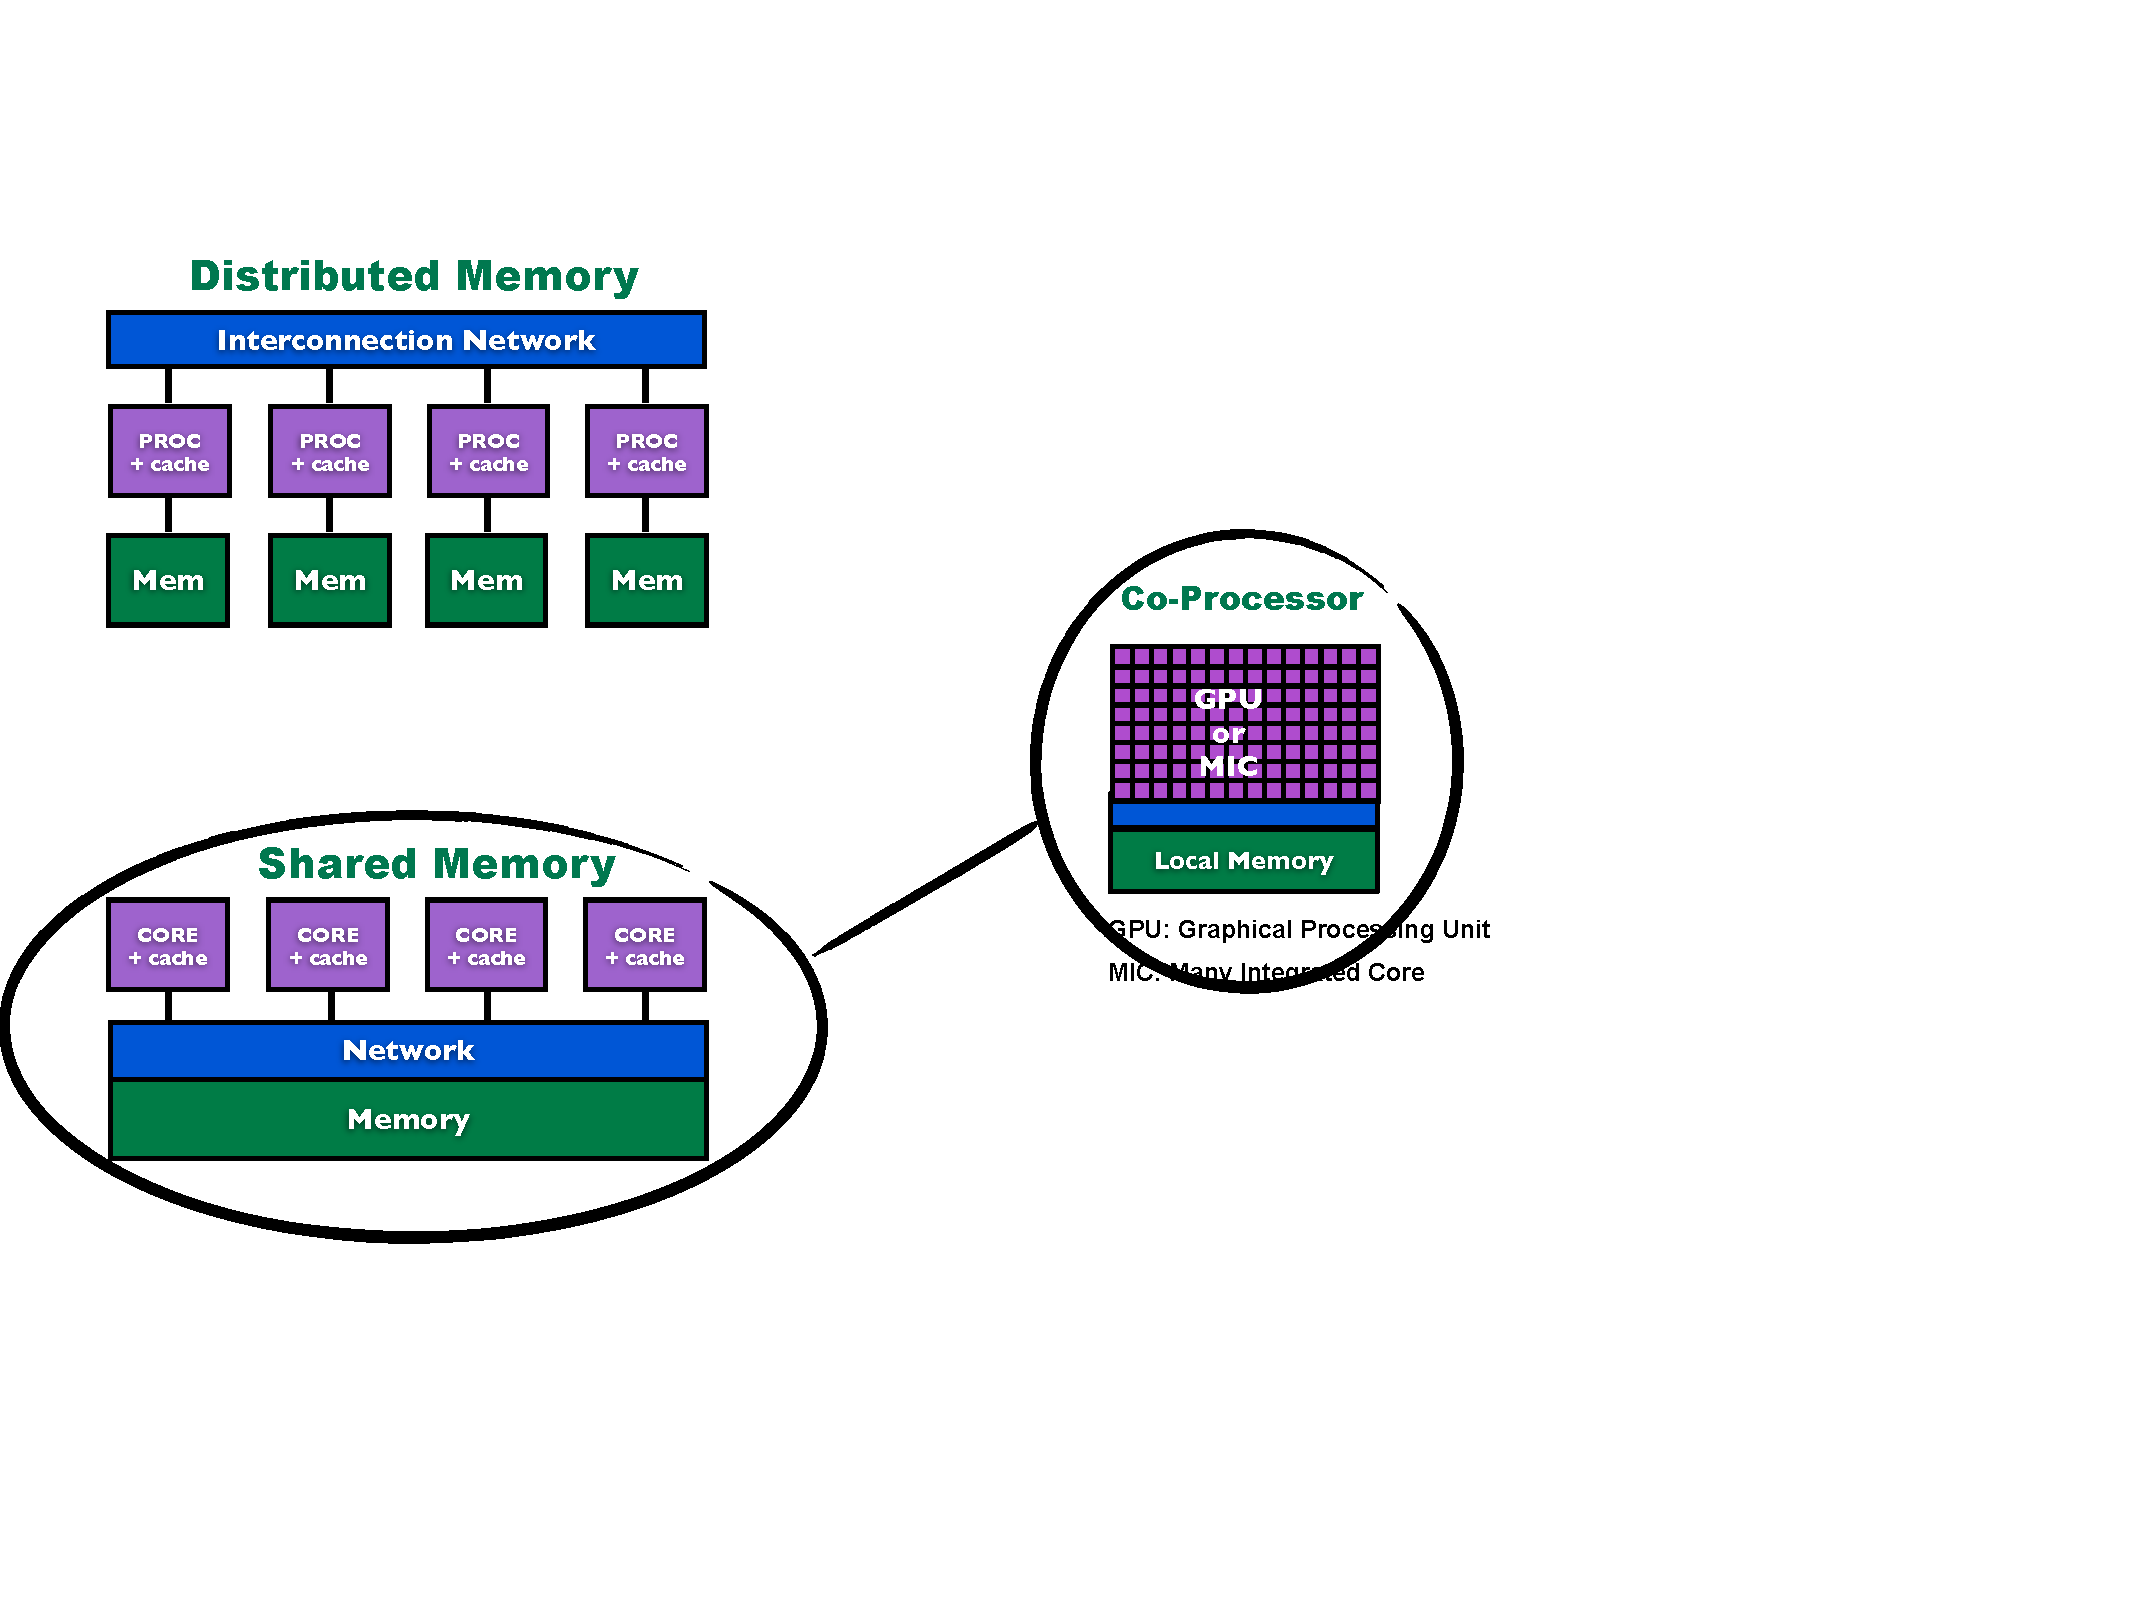
\includegraphics[width=0.95\textwidth]
{../common/pics/hardware/ParallelHardware2.pdf}
\end{frame}

\begin{frame}{A Server or Cluster}
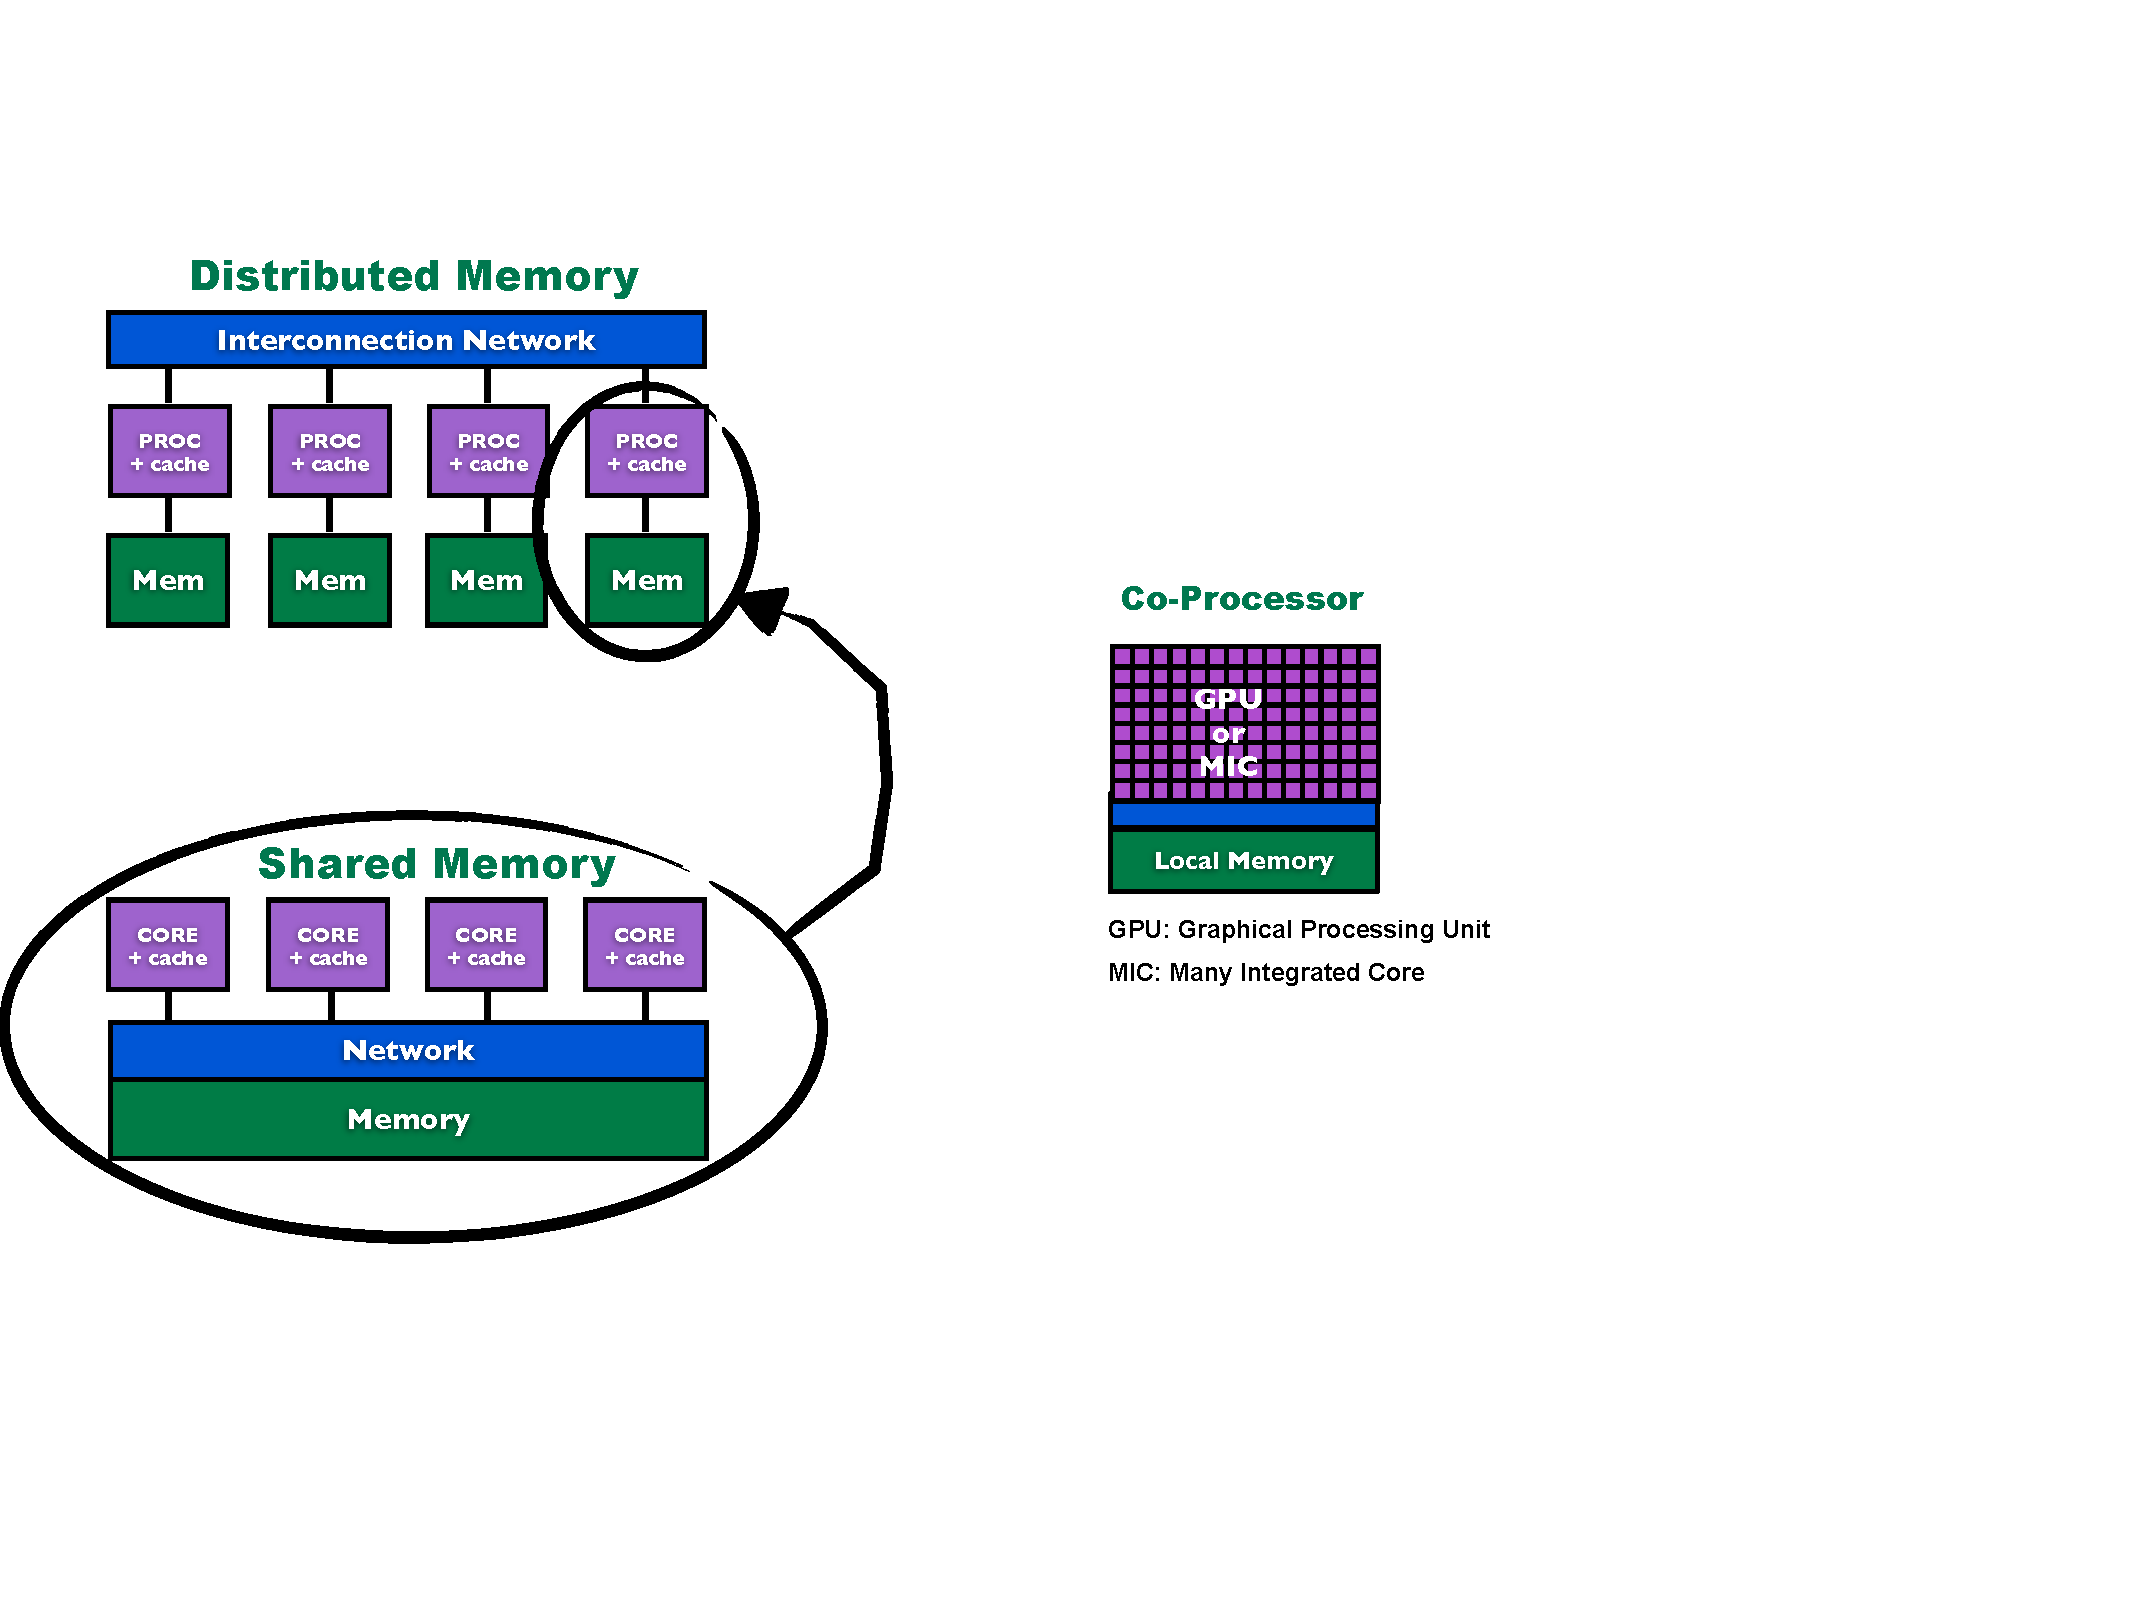
\includegraphics[width=0.95\textwidth]
{../common/pics/hardware/ParallelHardware3.pdf}
\end{frame}

\begin{frame}{Server to Supercomputer}
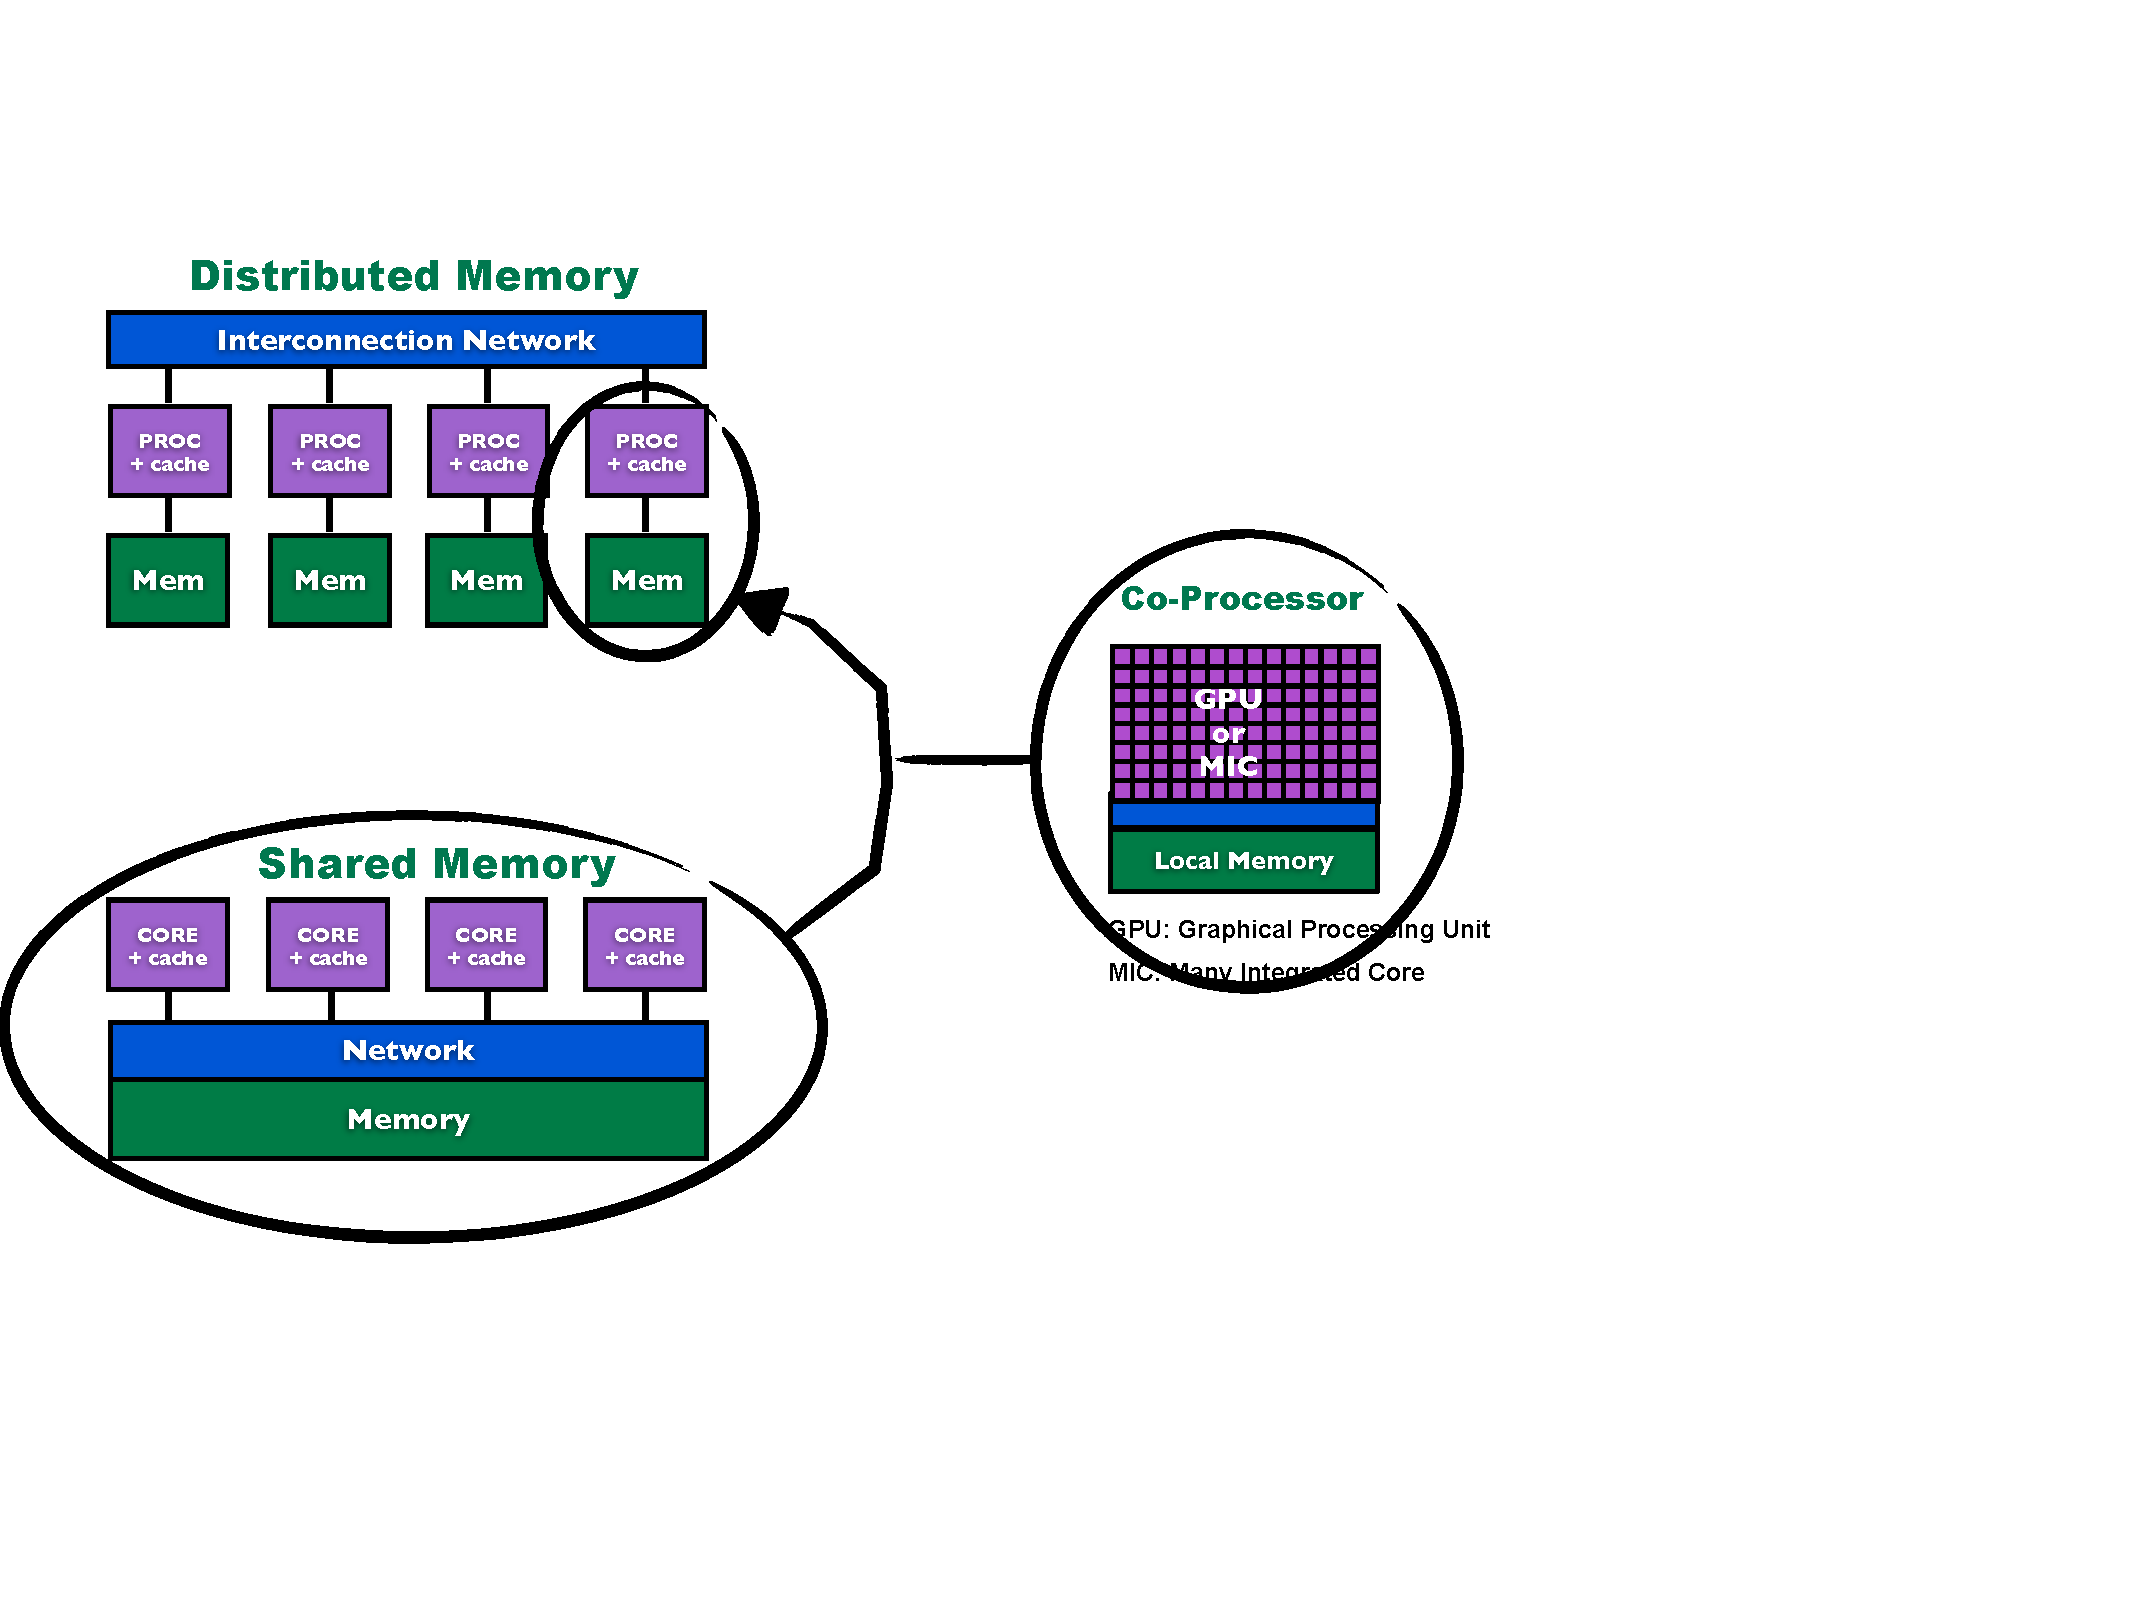
\includegraphics[width=0.95\textwidth]
{../common/pics/hardware/ParallelHardware4.pdf}
\end{frame}

\begin{frame}{Knowing the Right Words}
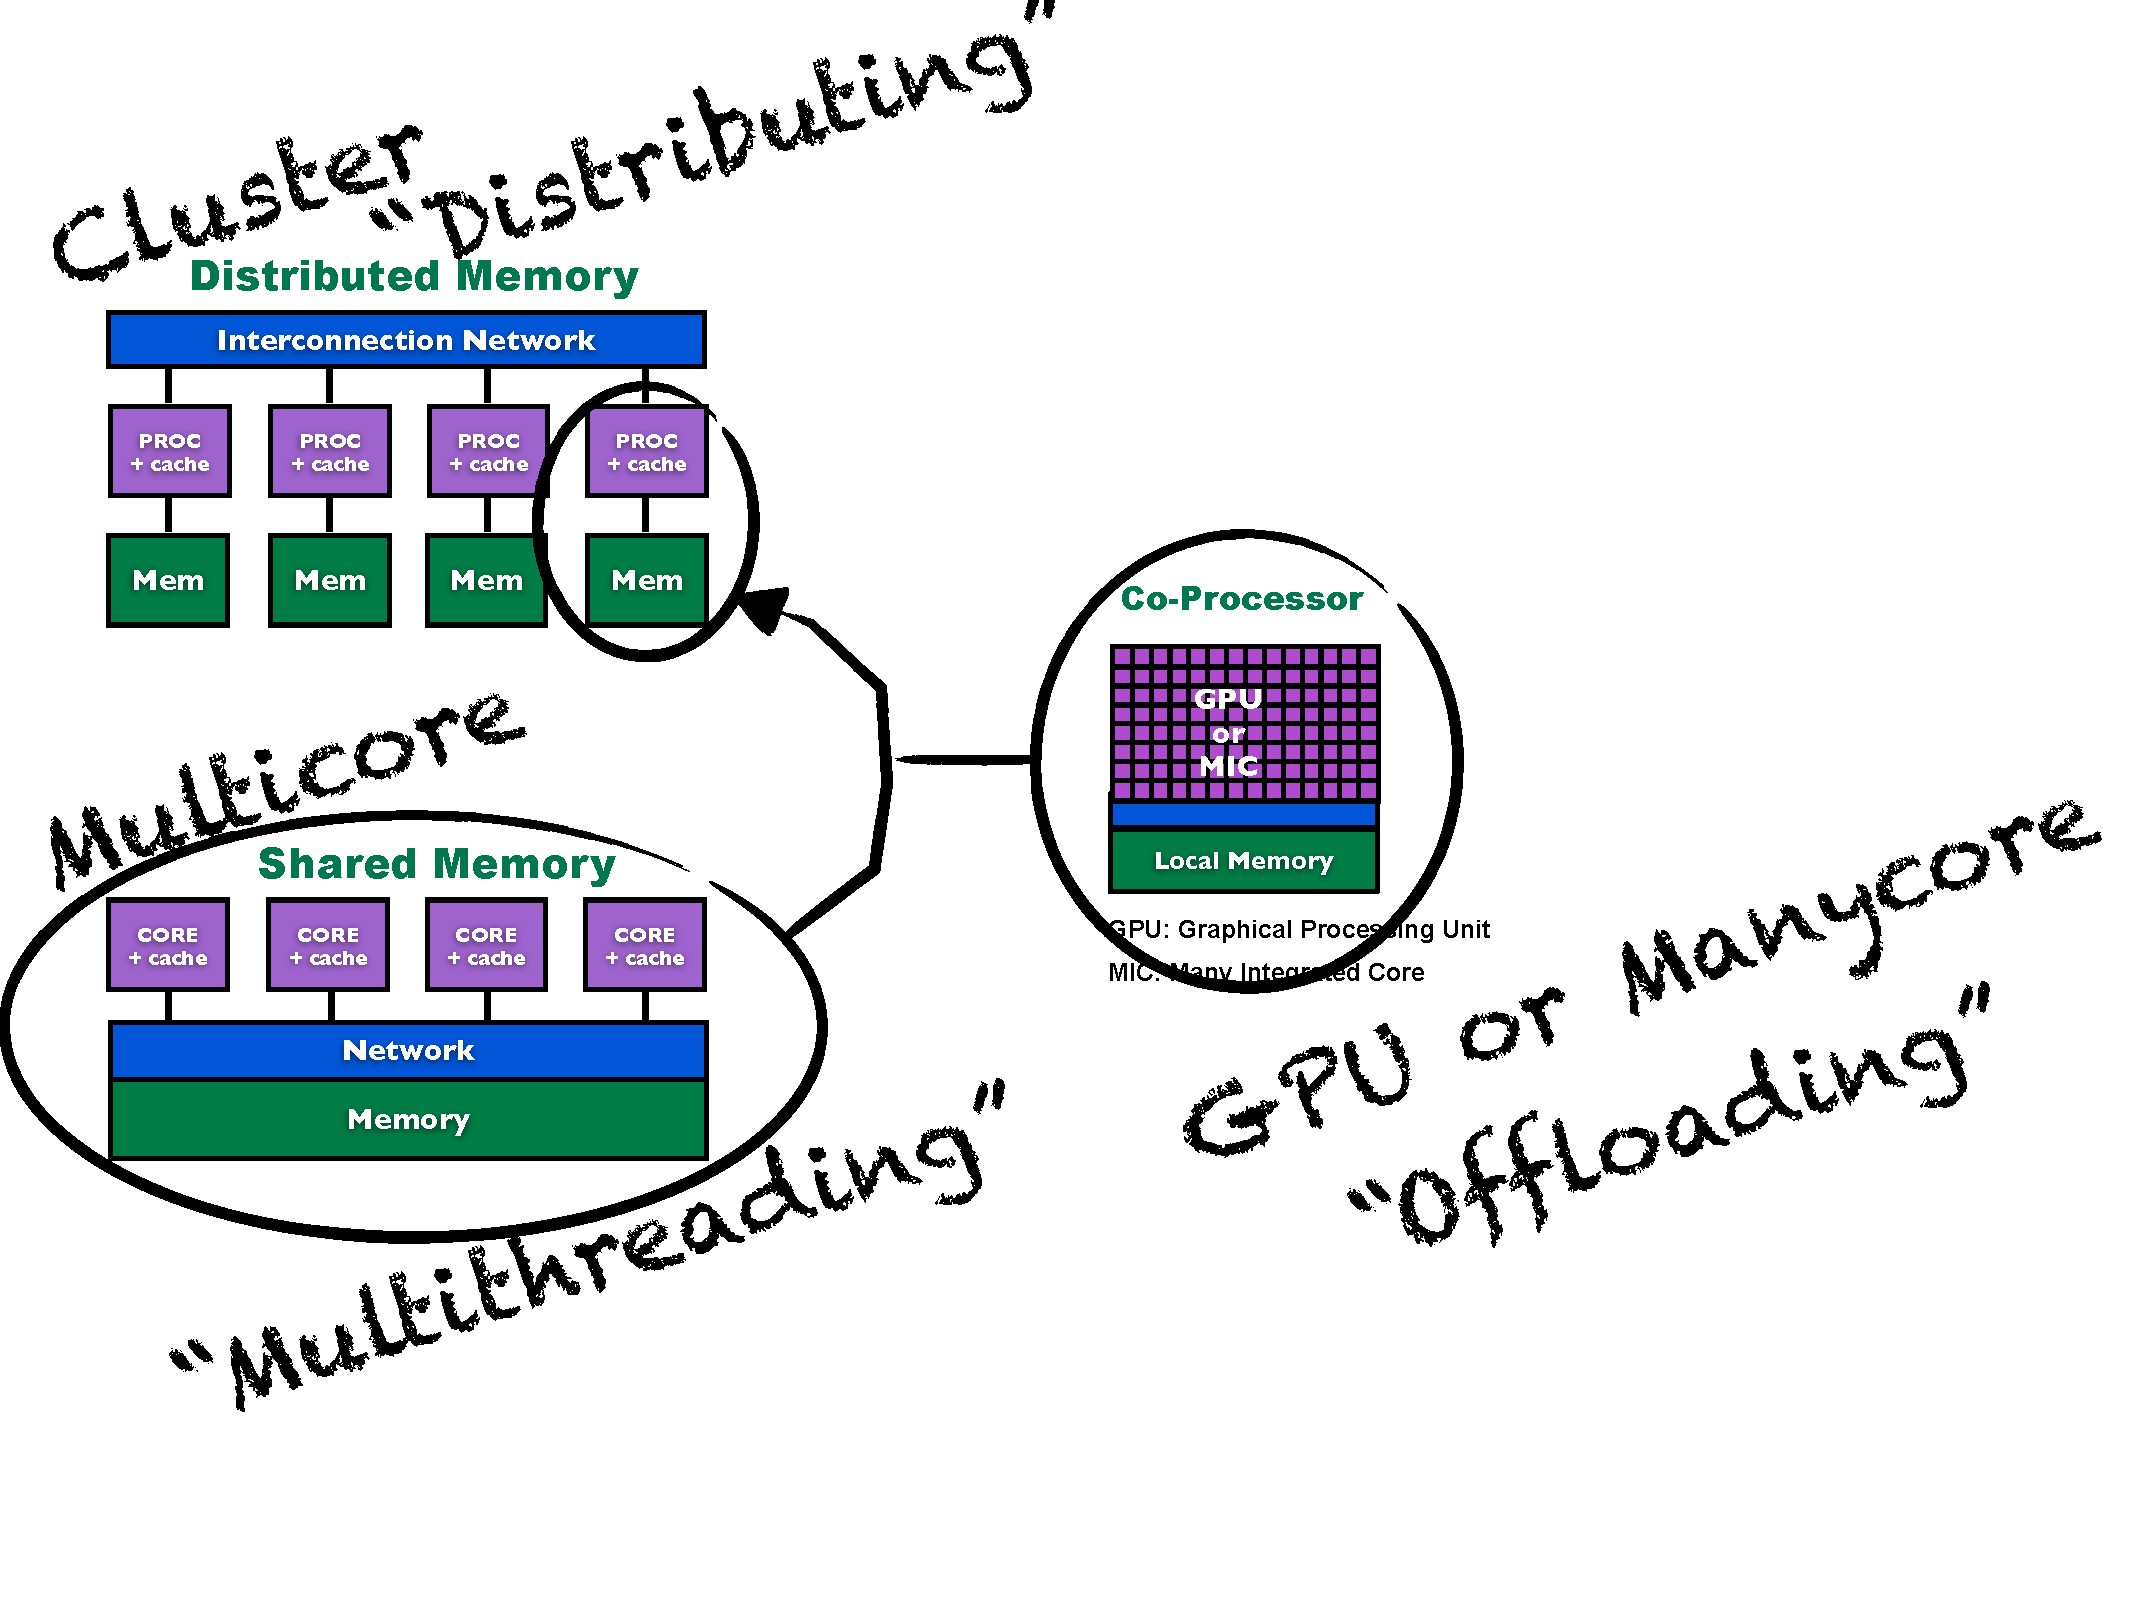
\includegraphics[width=0.95\textwidth]
{../common/pics/hardware/ParallelHardware5.pdf}
\end{frame}

\subsection{A Quick Overview of Parallel Software}
\makesubcontentsslidessec

\begin{frame}{``Native'' Programming Models and Tools}
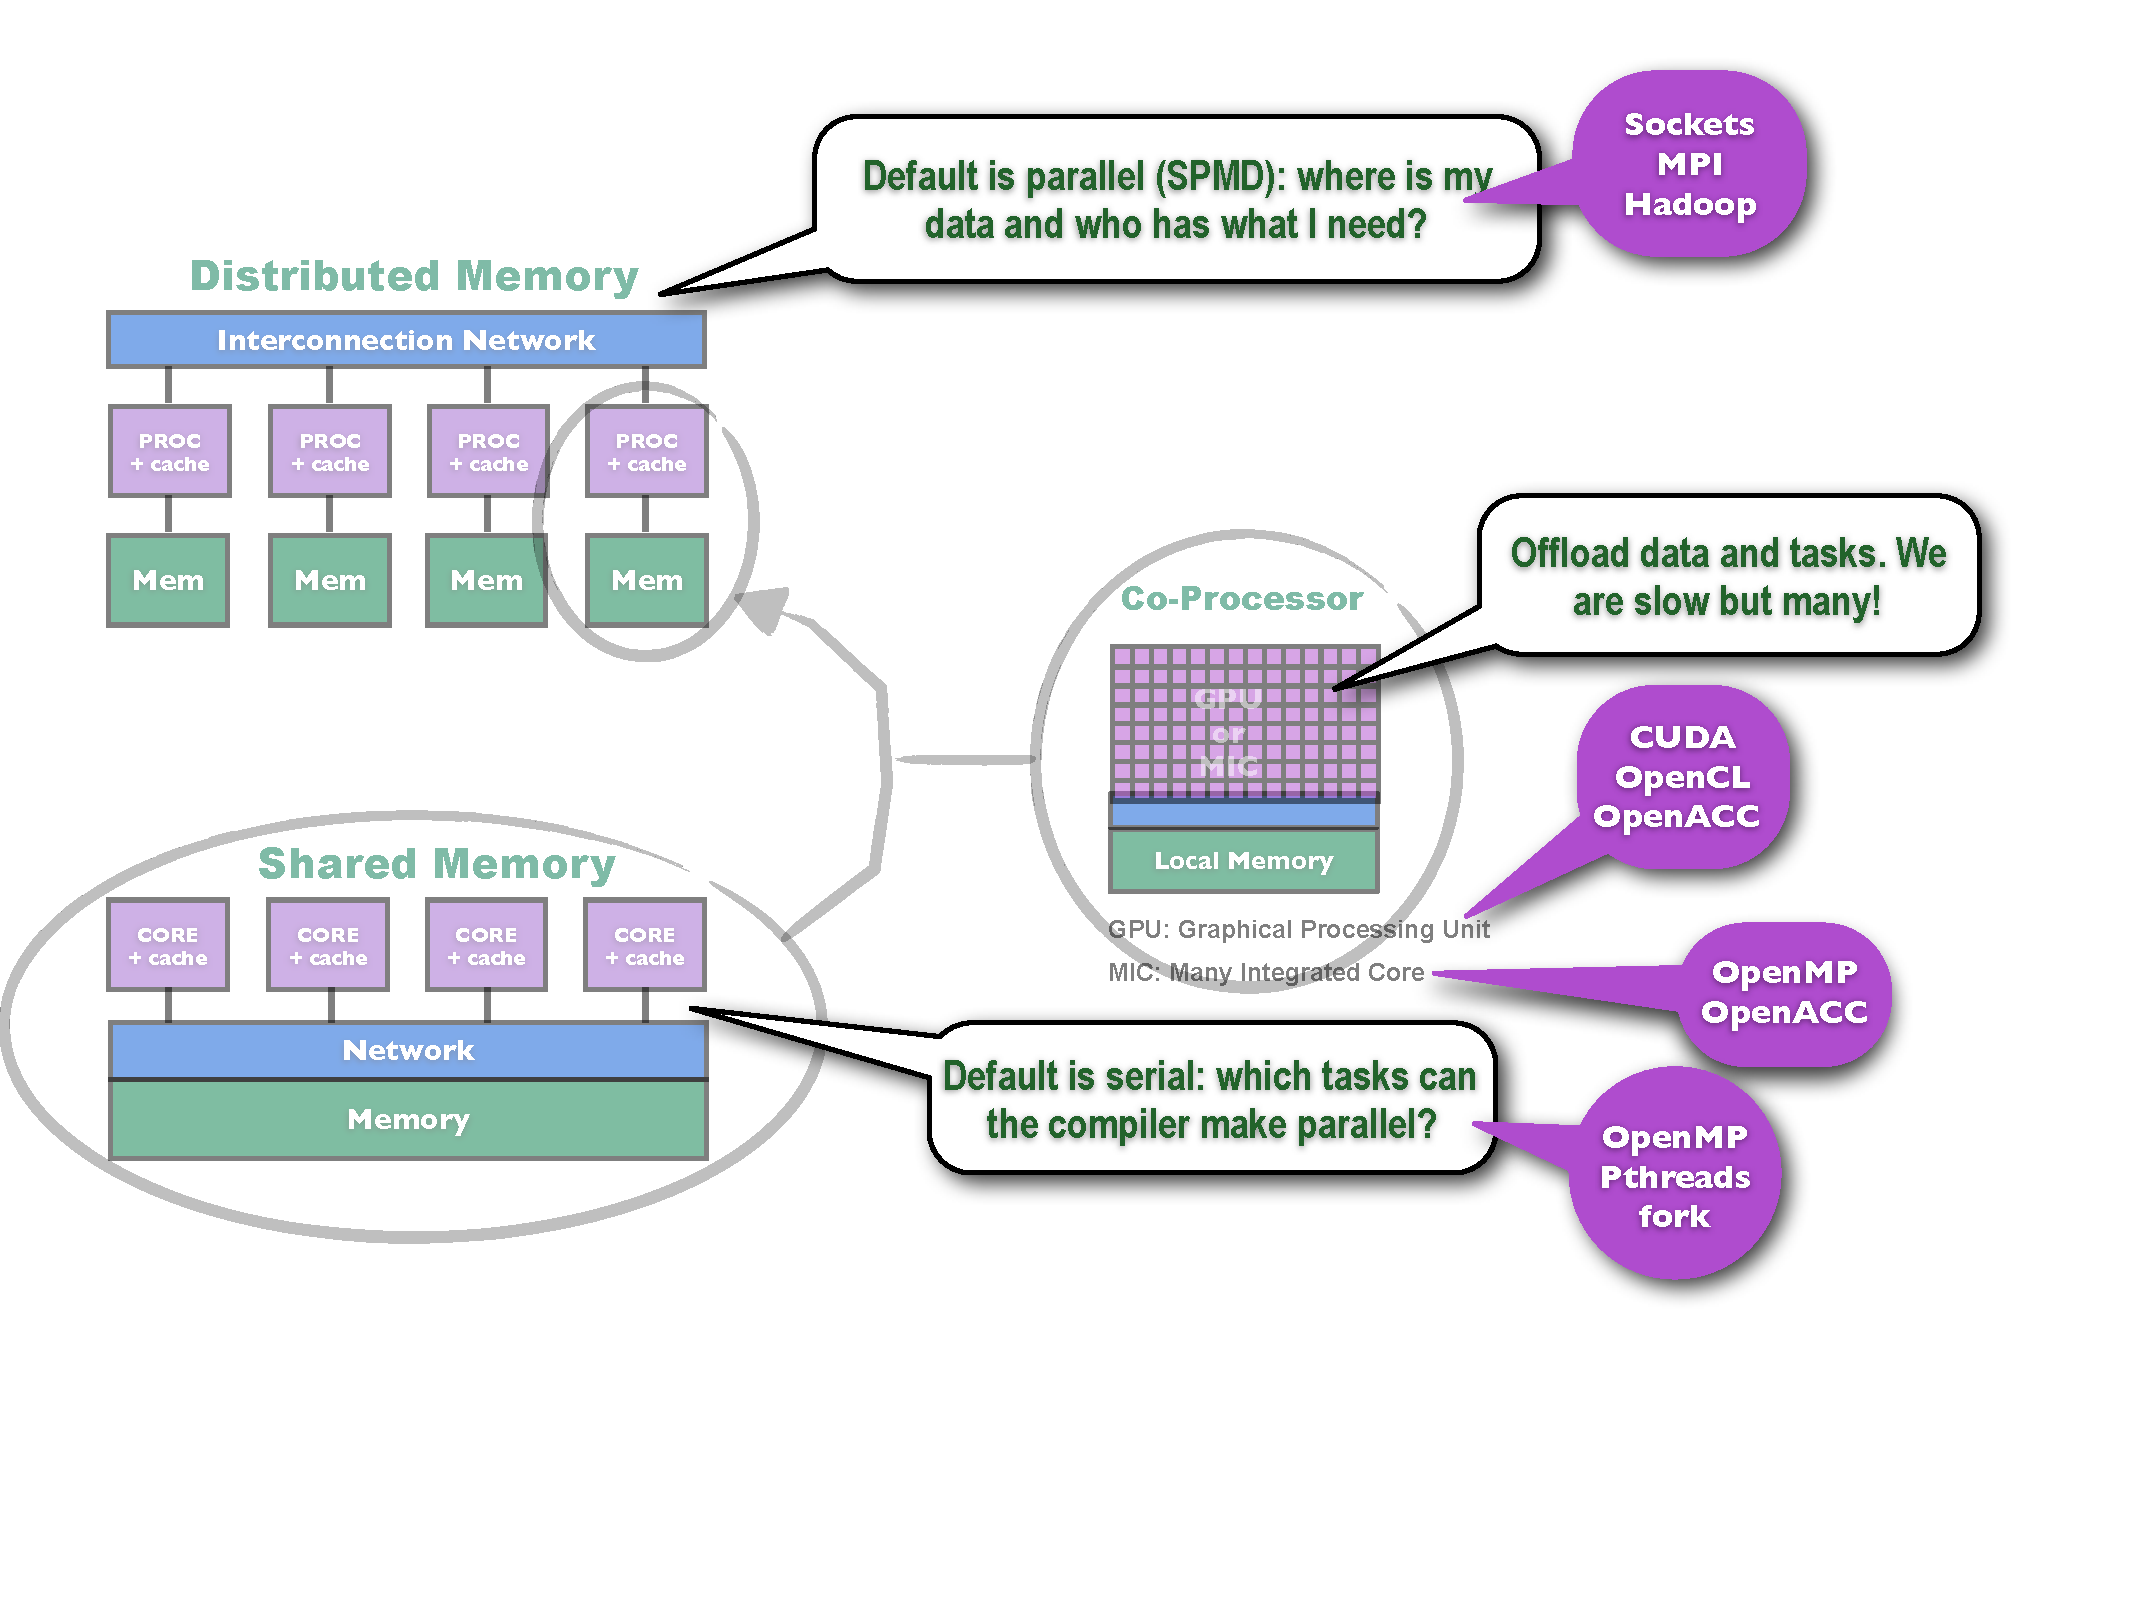
\includegraphics[width=0.95\textwidth]
{../common/pics/hardware/ParallelHardware6.pdf}
\end{frame}

\begin{frame}{30+ Years of Parallel Computing Research}
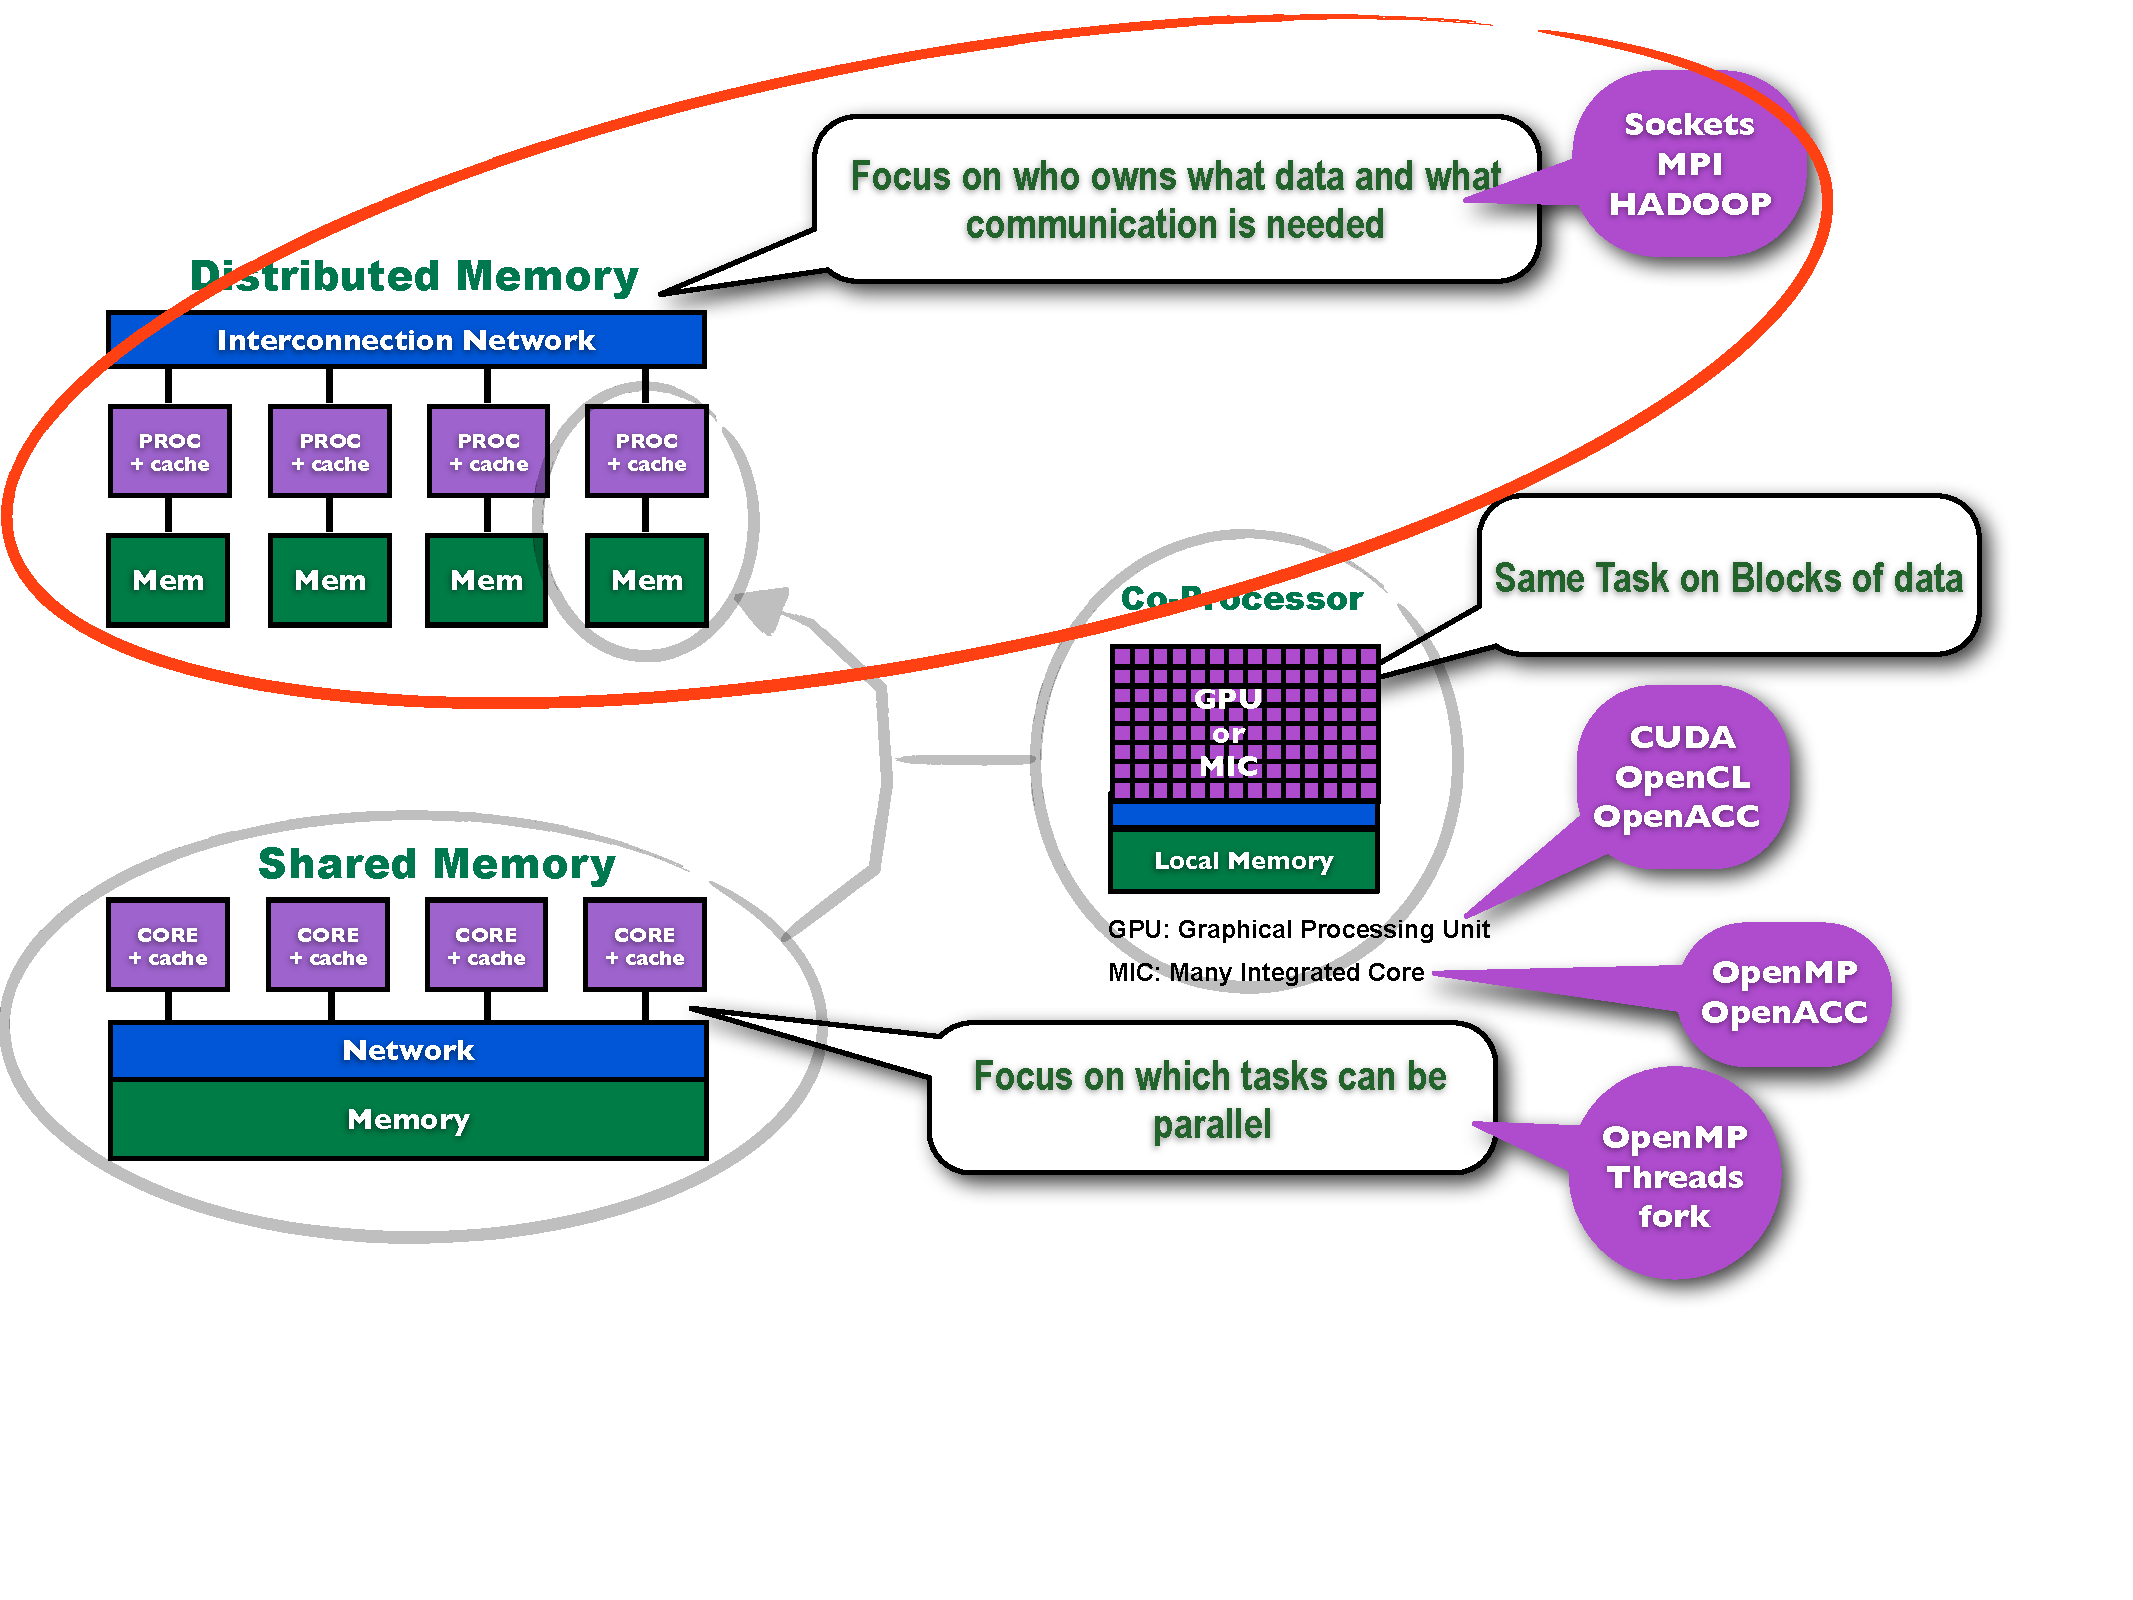
\includegraphics[width=0.95\textwidth]
{../common/pics/hardware/ParallelHardware7.pdf}
\end{frame}

\begin{frame}{Last 10 years of Advances}
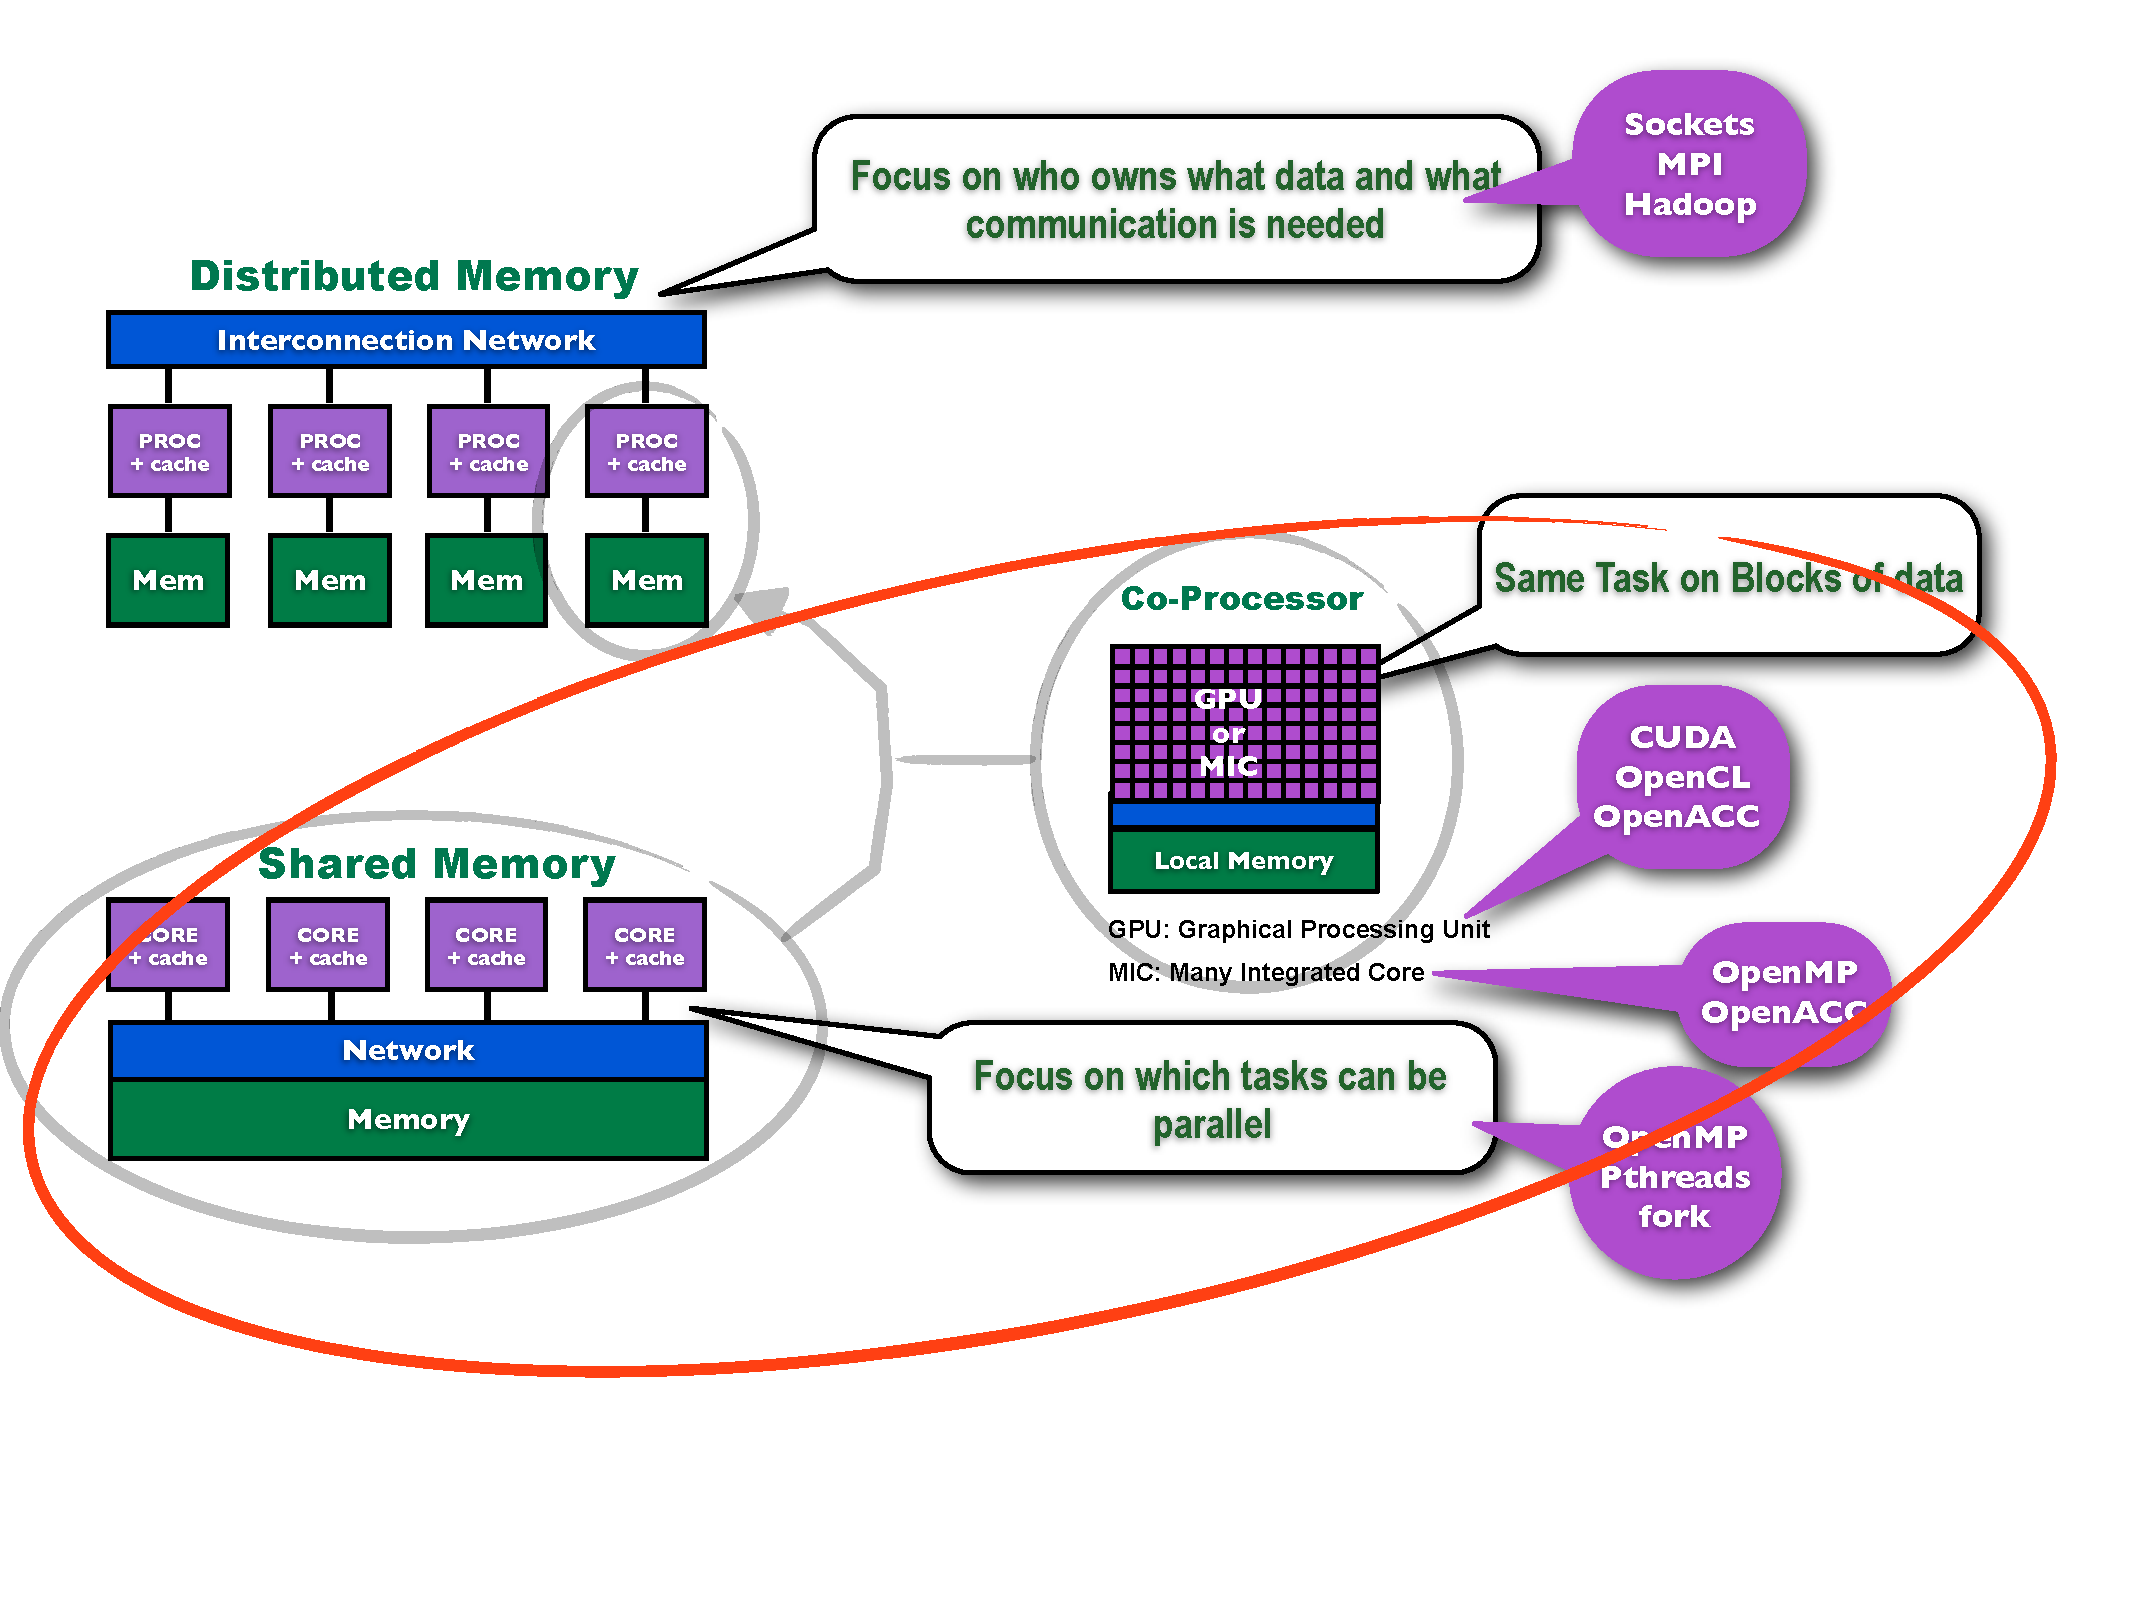
\includegraphics[width=0.95\textwidth]
{../common/pics/hardware/ParallelHardware8.pdf}
\end{frame}

\begin{frame}{Putting It All Together Challenge}
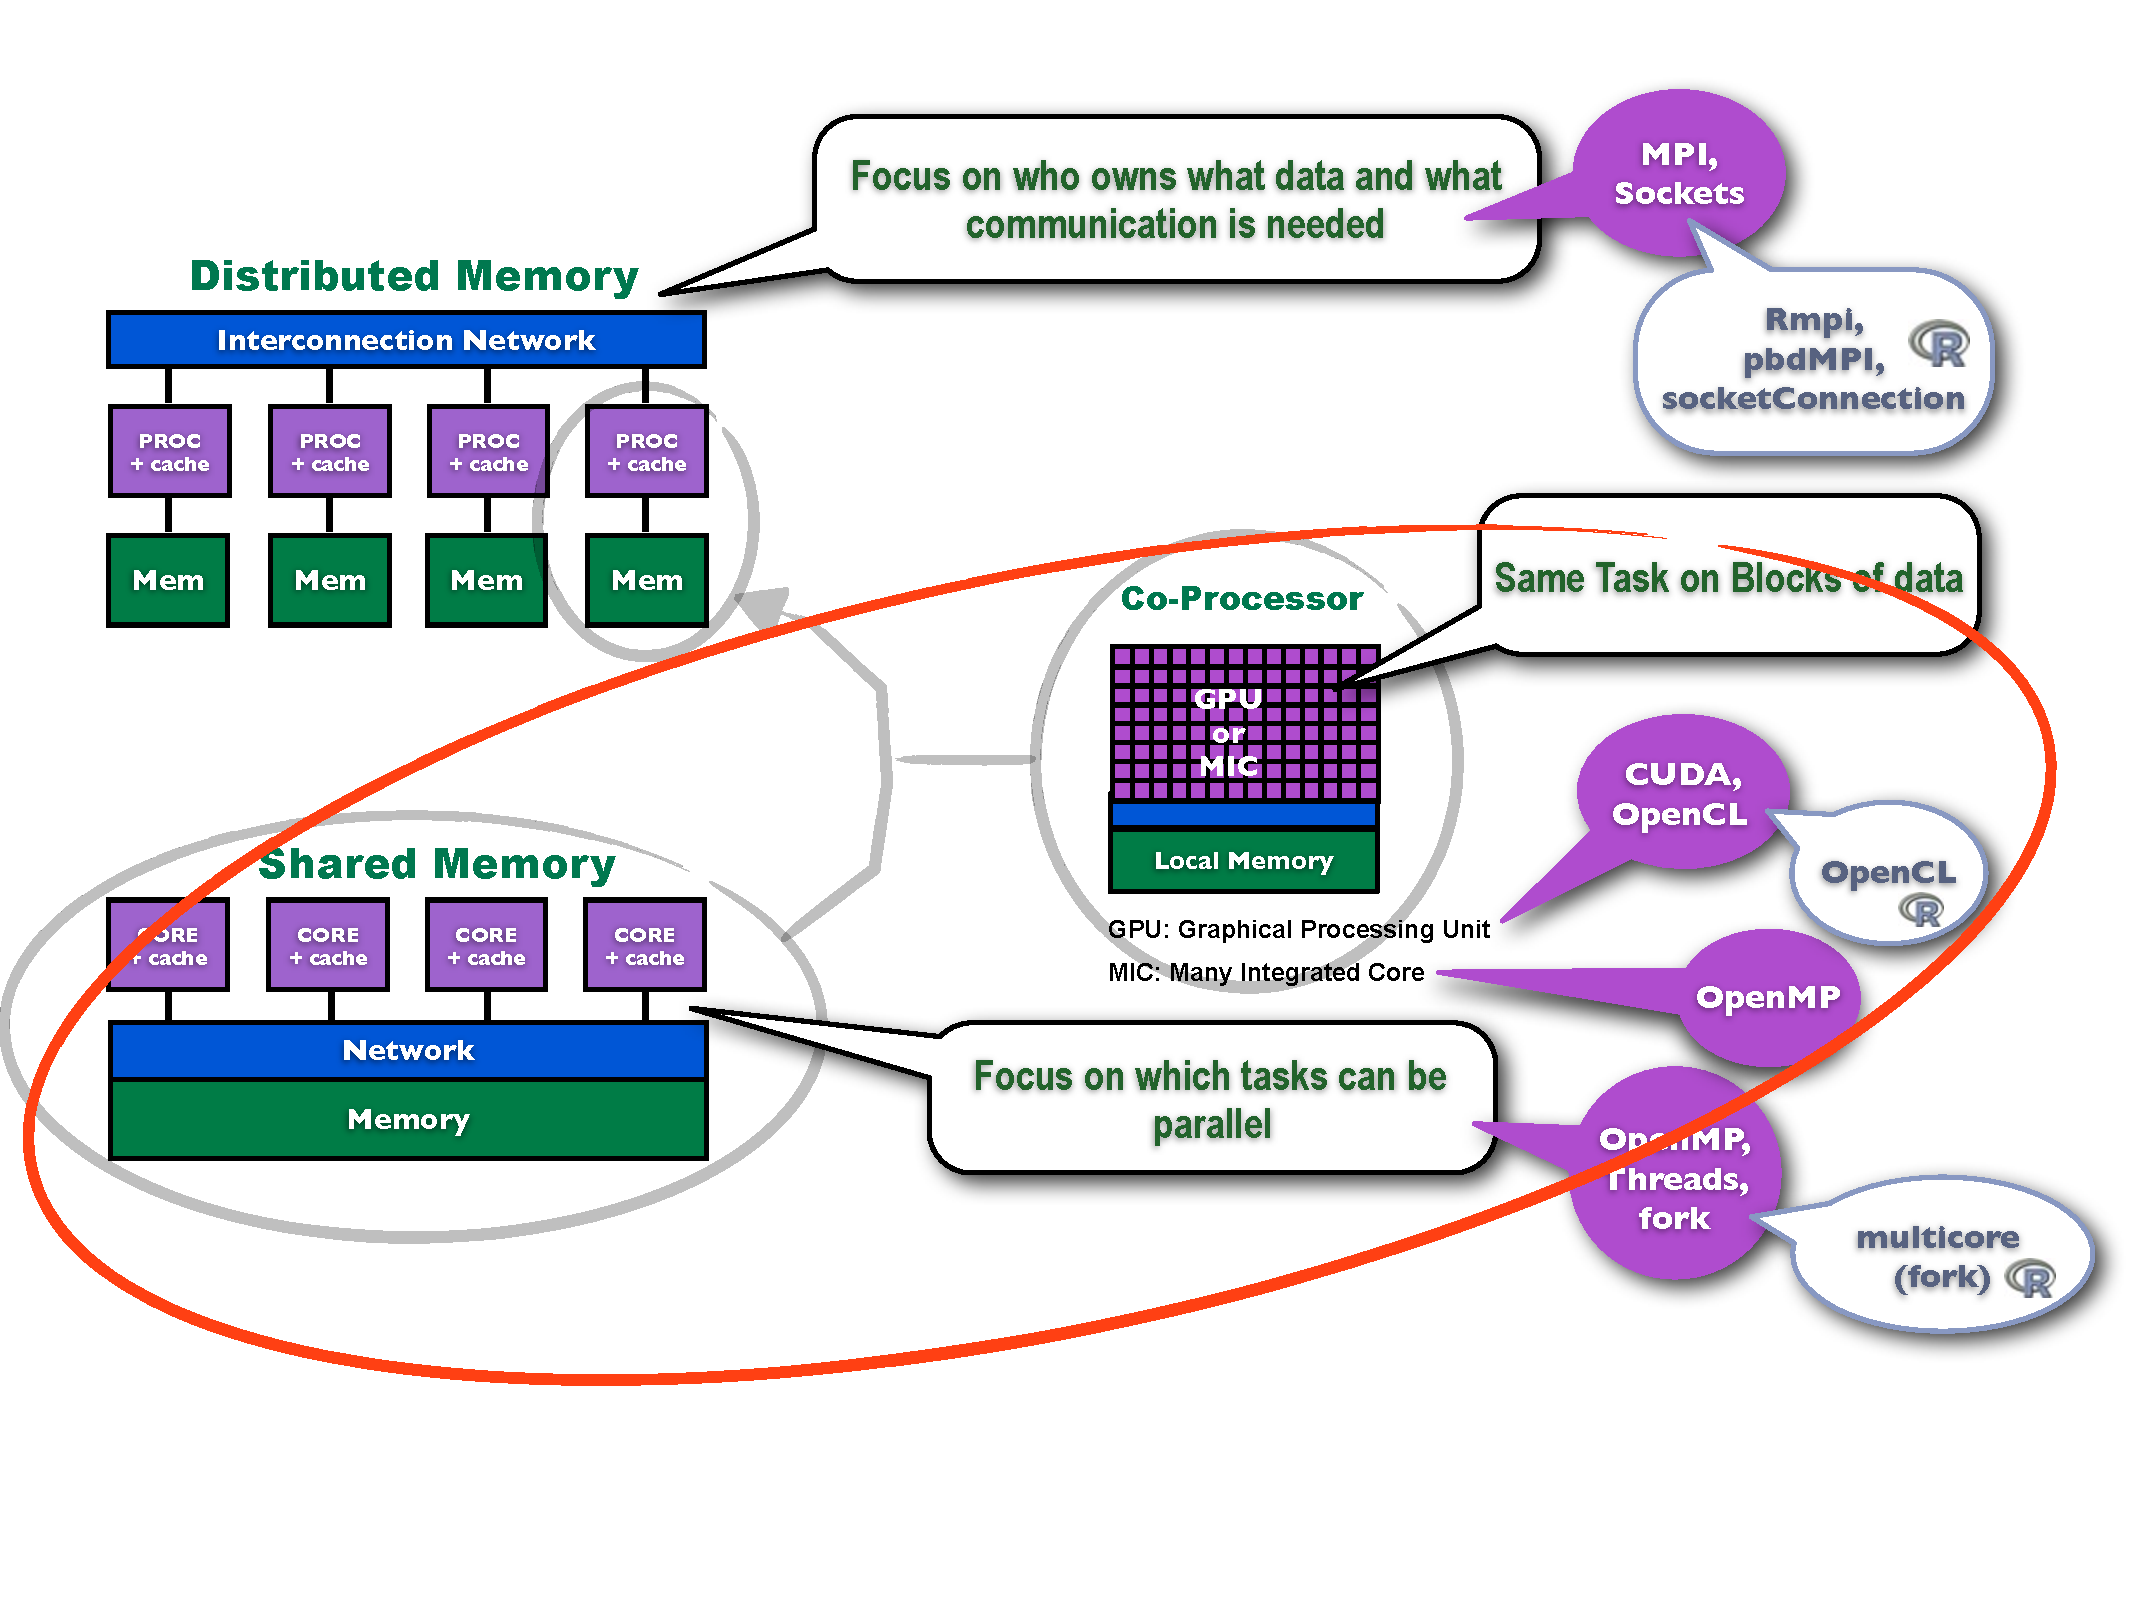
\includegraphics[width=0.95\textwidth]
{../common/pics/hardware/ParallelHardware9.pdf}
\end{frame}

\begin{frame}{Distributed Programming Works in Shared Memory}
\includegraphics[width=0.95\textwidth]
{../common/pics/hardware/ParallelHardware29.pdf}
\end{frame}

\begin{frame}{R Interfaces to Low-Level Native Tools}
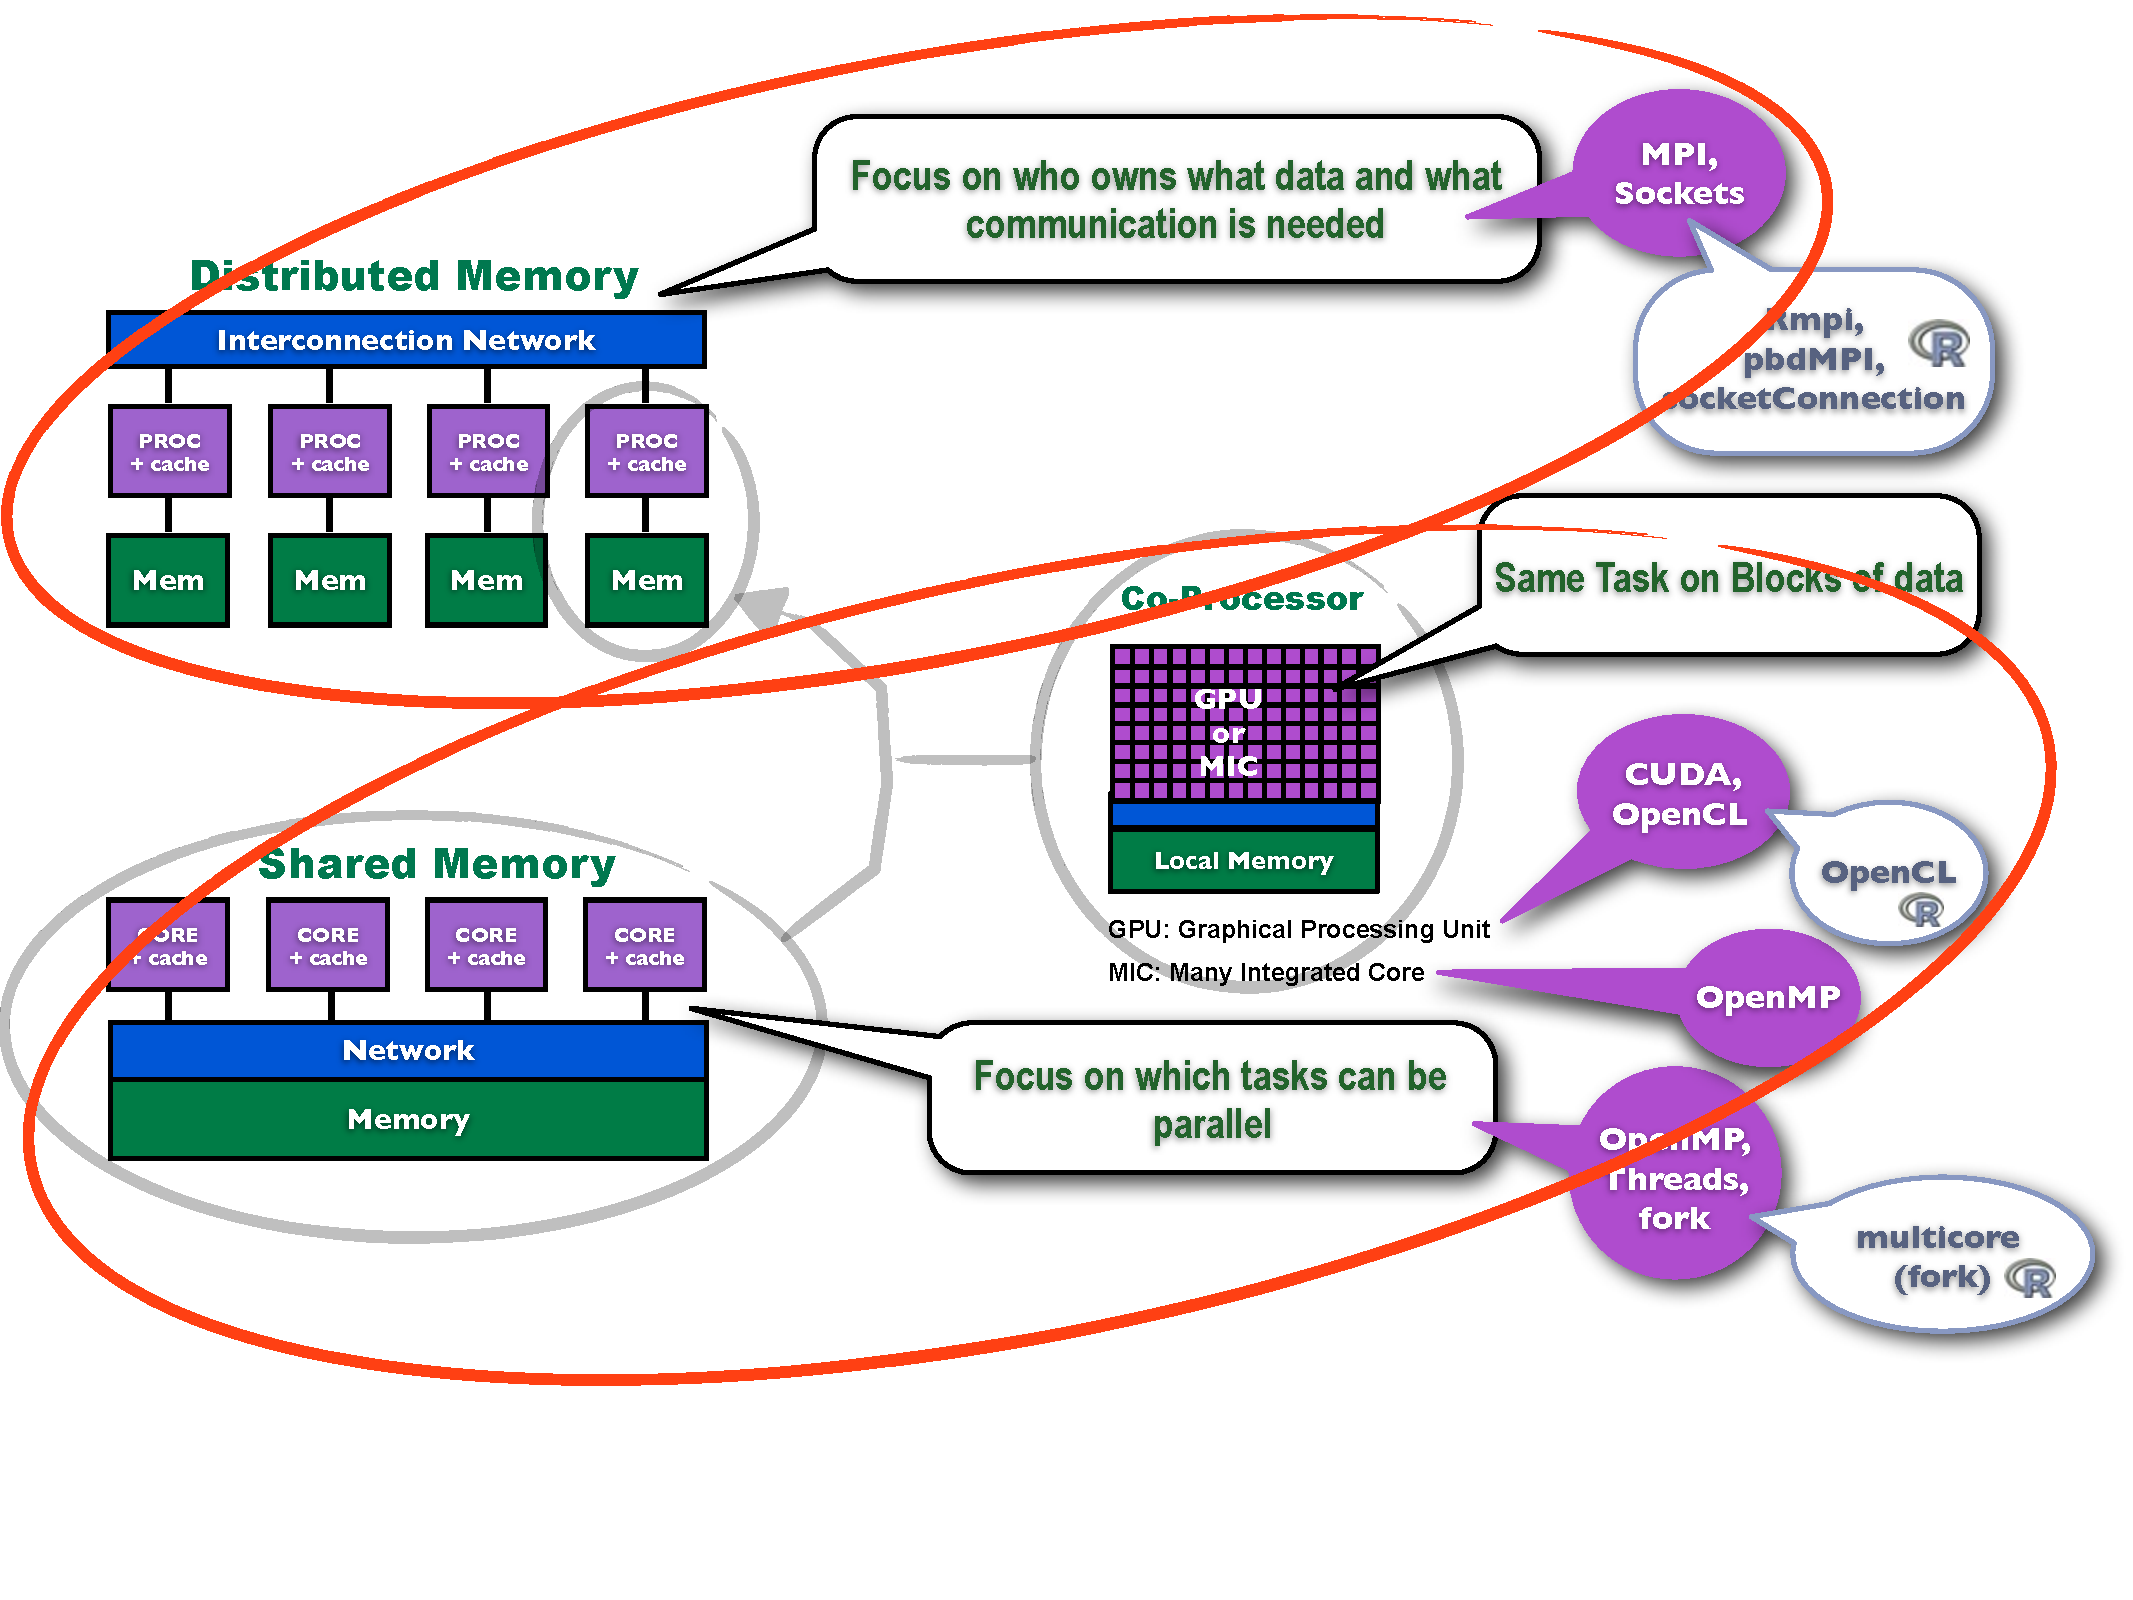
\includegraphics[width=0.95\textwidth]
{../common/pics/hardware/ParallelHardware10.pdf}
\end{frame}

\begin{frame}{Scalable Libraries}
\includegraphics[width=0.95\textwidth]
{../common/pics/hardware/ParallelHardware25.pdf}
\end{frame}

\begin{frame}{R and \pbdR Interfaces to HPC Libraries}
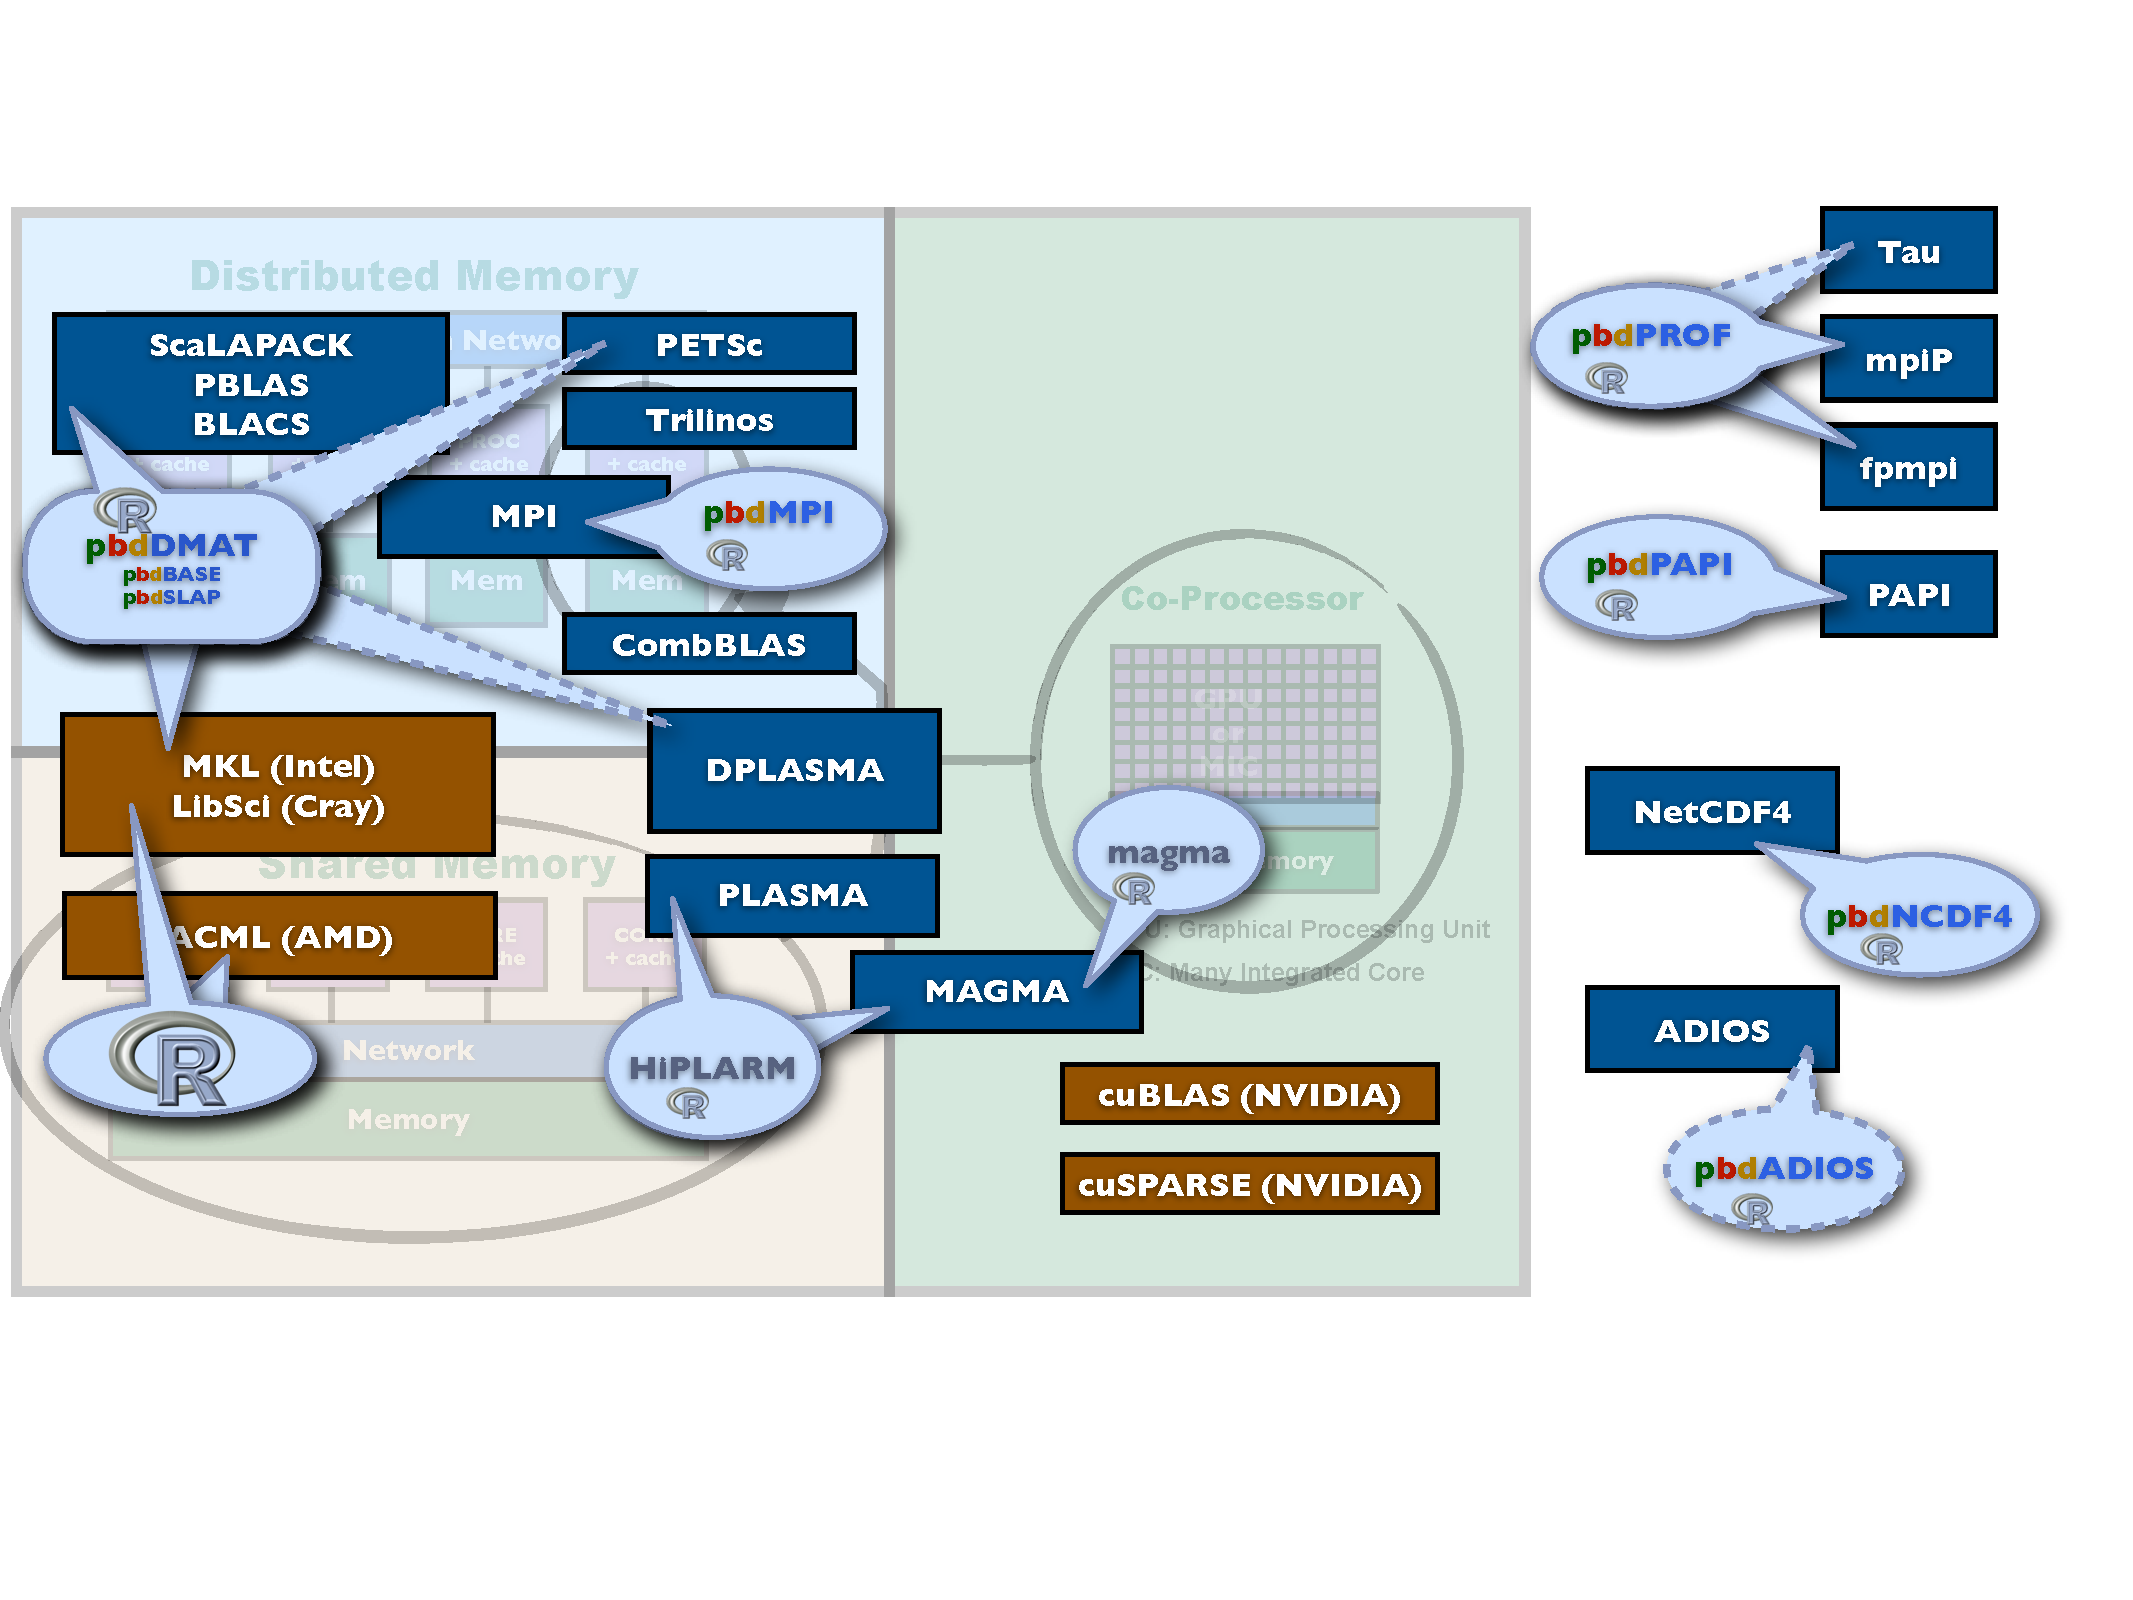
\includegraphics[height=\textheight]
{../common/pics/hardware/ParallelHardware26.pdf}
\end{frame}


\subsection{Cluster Computer Architectures}
\makesubcontentsslidessec

\begin{frame}{Parallel Computing before Multicore}
\begin{minipage}{8.0cm}
  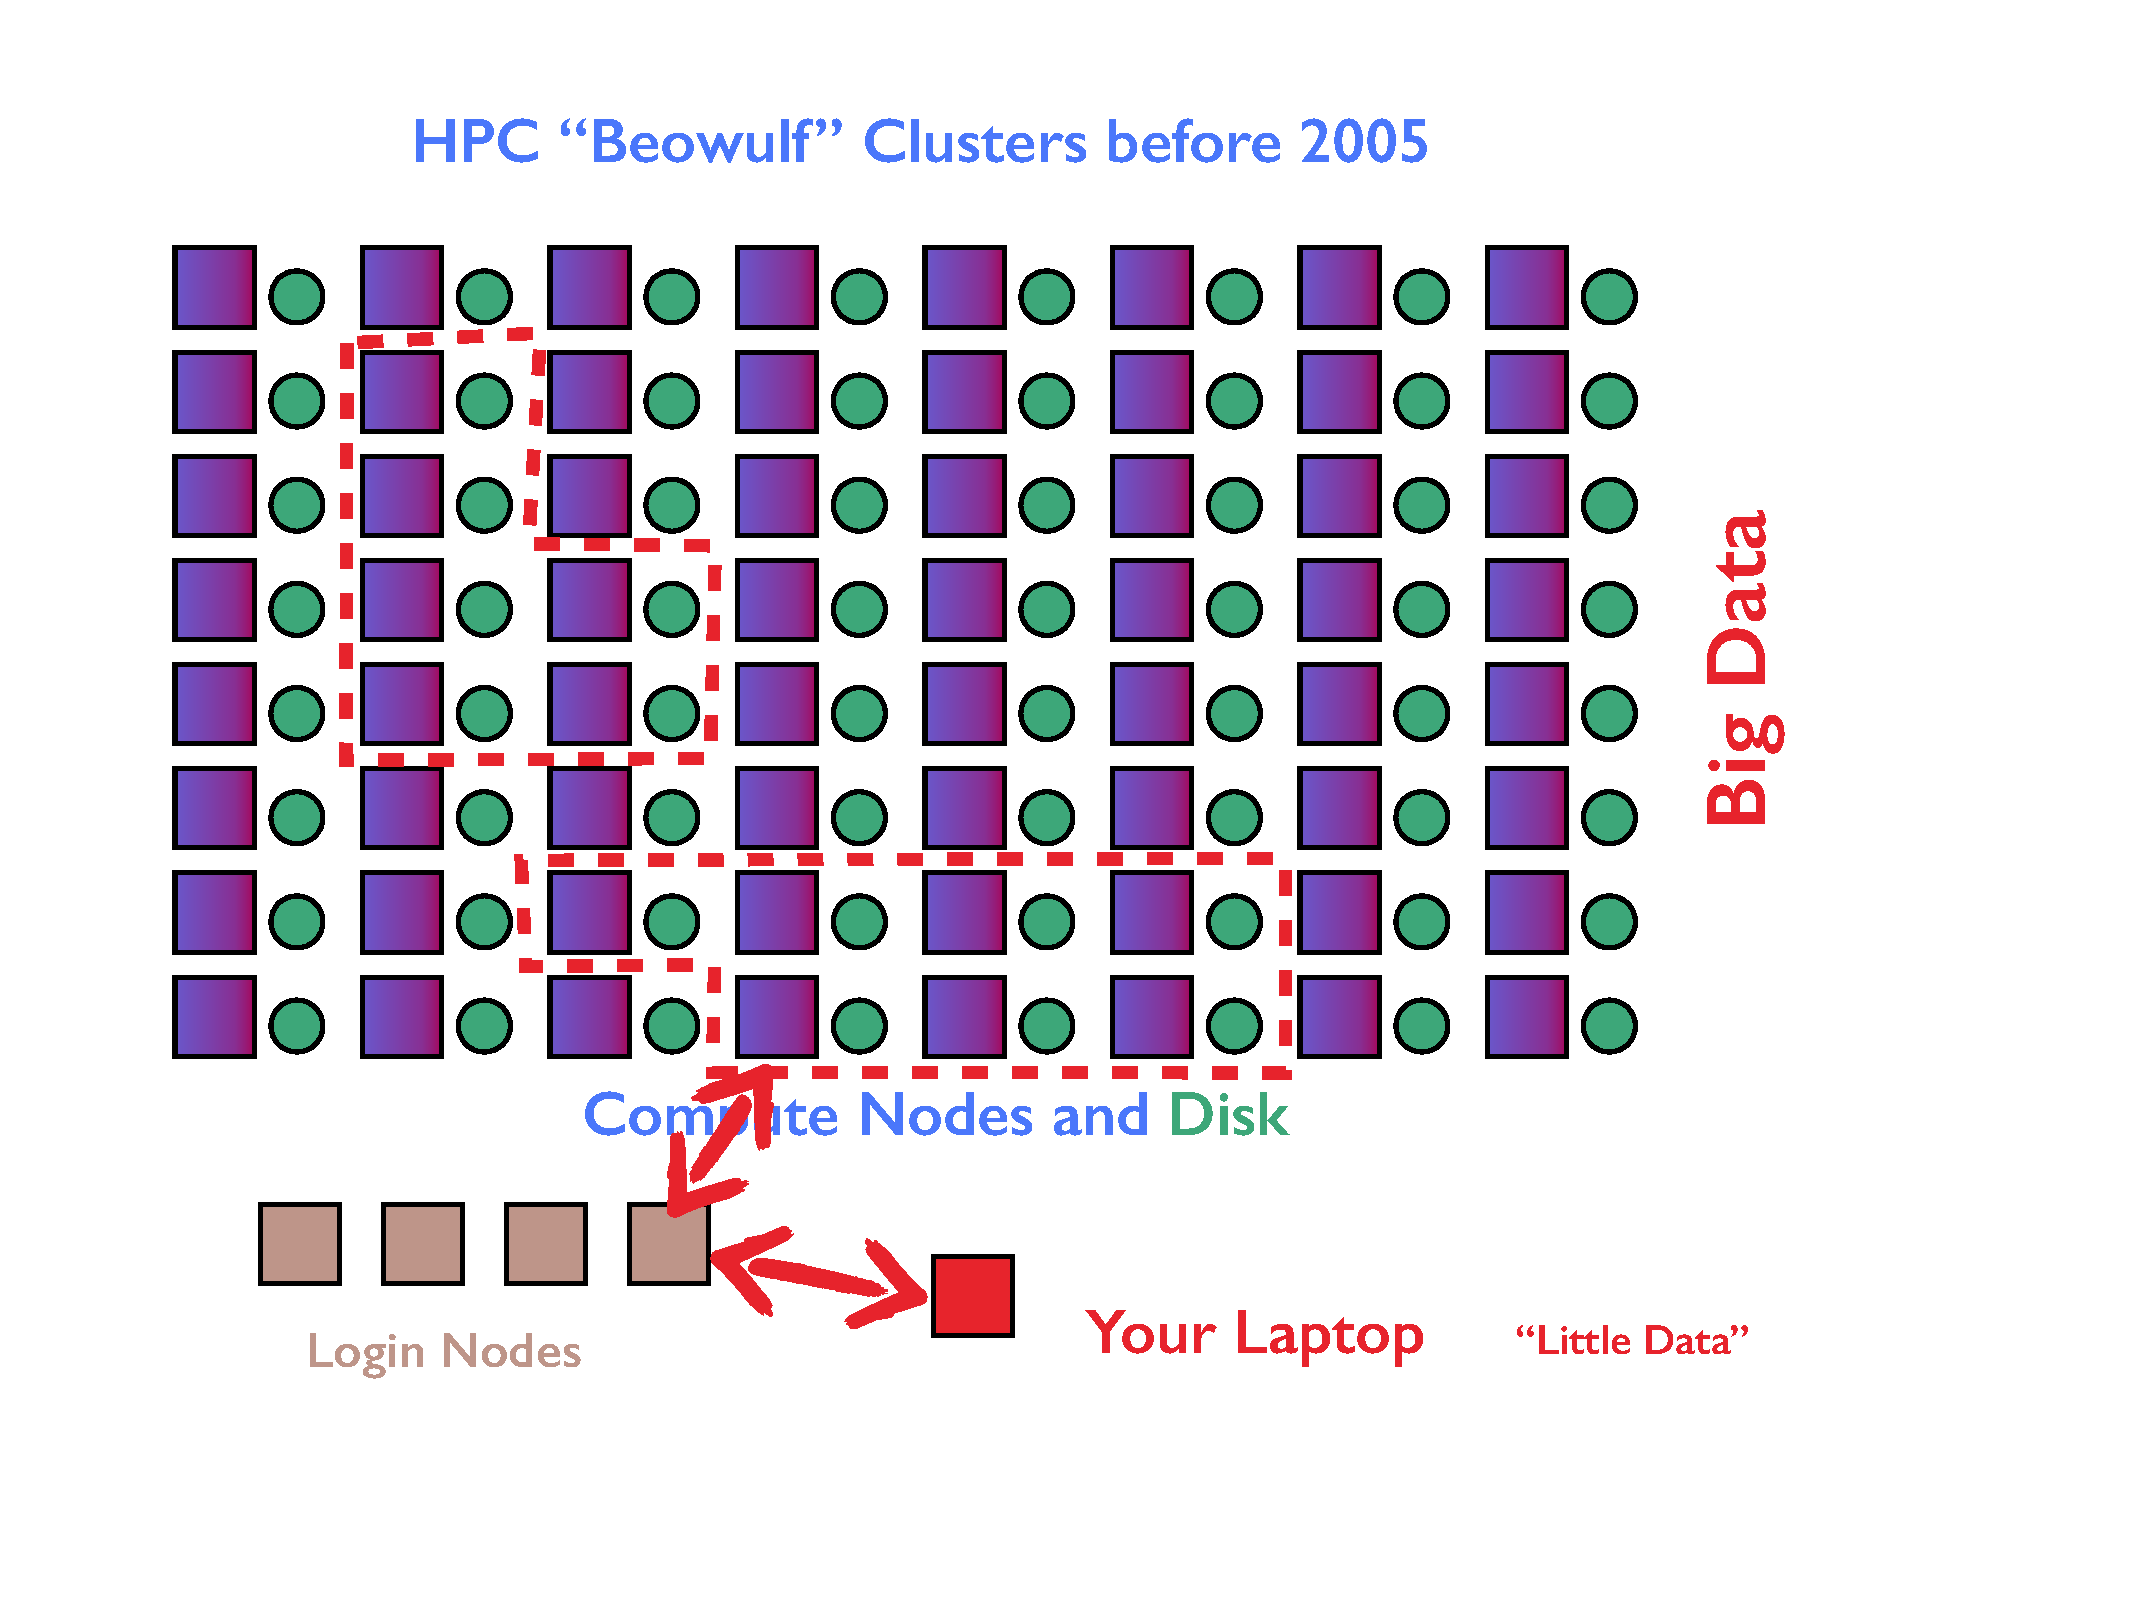
\includegraphics[trim=3cm 0cm 0cm 0cm,clip=true,height=0.9\textheight]
  {../common/pics/hardware/ParallelHardware22.pdf}\hfill
\end{minipage}
\hspace{1ex}
\begin{minipage}{3.6cm}\small
  \begin{block}{Software Developments:}\pause
    \scriptsize MPI is mature, Map-Reduce emerges \\[1ex]
    Parallel Libraries: PBLAS, ScaLAPACK, PETSc, etc. \\[1ex]
    Resource Manager: PBS mature, HADOOP emerges
  \end{block}
\end{minipage}
\end{frame}

\begin{frame}{Multicore Emerges and Clusters become Diskless}
\begin{minipage}{8.0cm}
  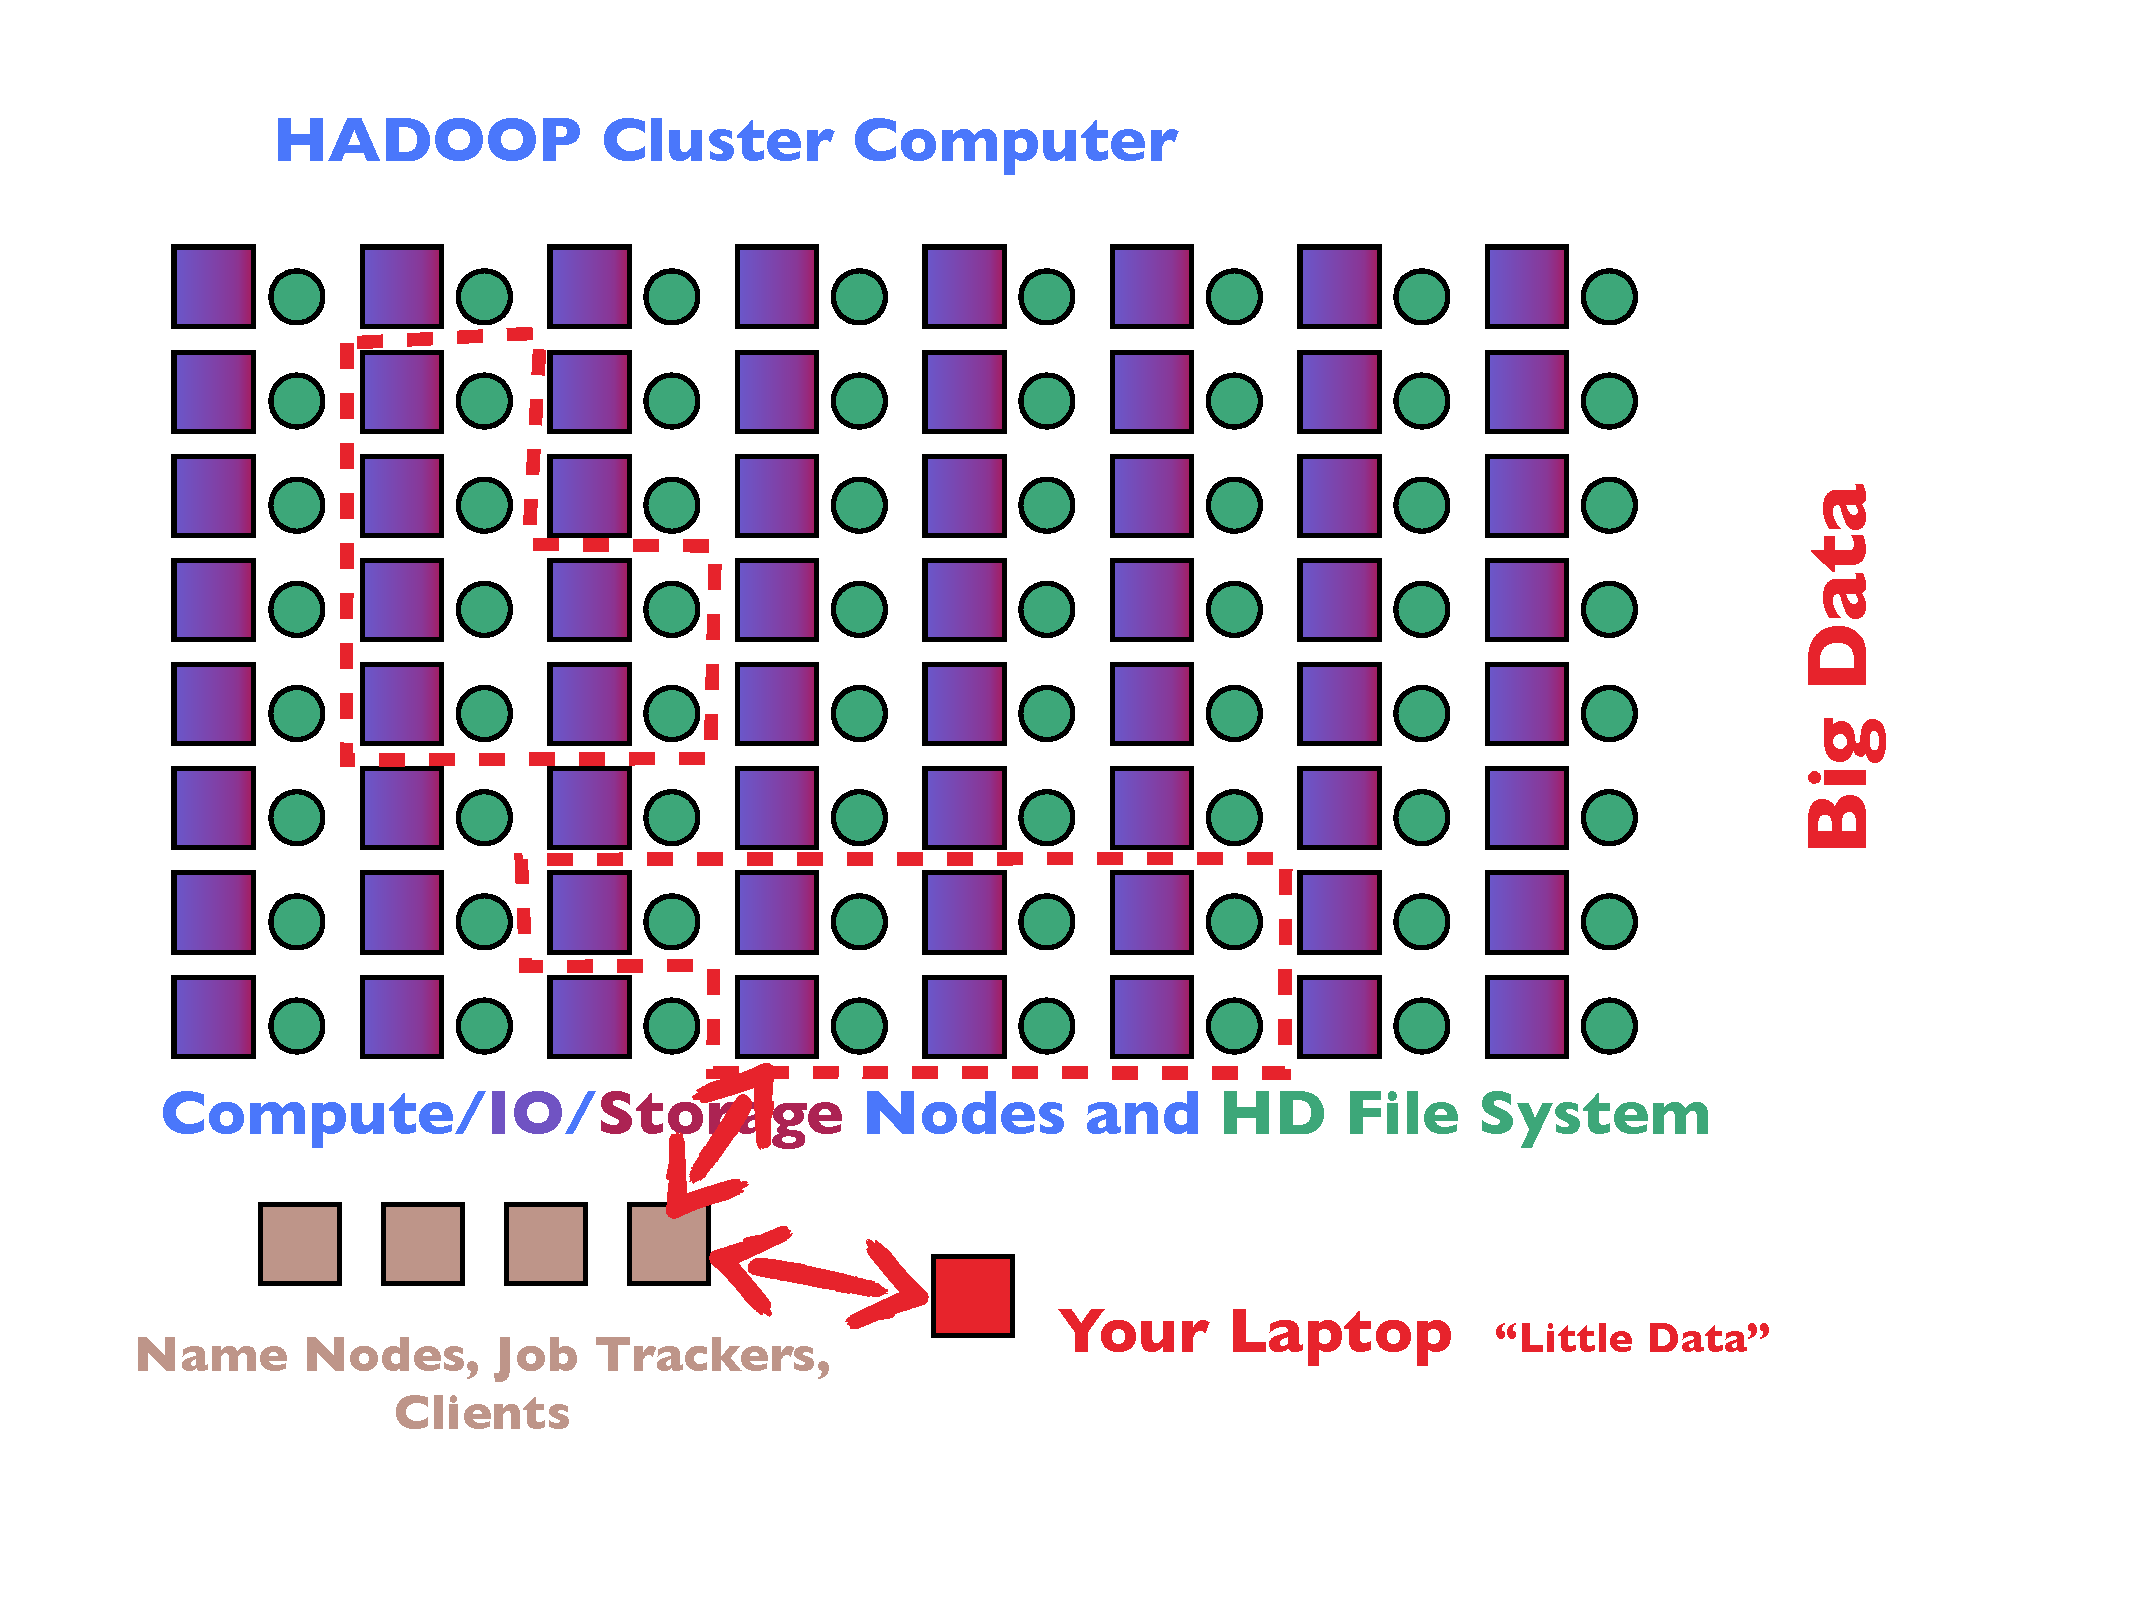
\includegraphics[trim=2cm 0cm 0cm 0cm,clip=true,height=0.8\textheight]
  {../common/pics/hardware/ParallelHardware23.pdf}
\end{minipage}
\begin{minipage}{3.7cm}\small
  \begin{block}{Software Developments}\pause
    \scriptsize OpenMP, CUDA, OpenCL, OpenACC \\[1ex]
    Libraries: PLASMA, MAGMA, CuBLAS
  \end{block}
\end{minipage}
\end{frame}

\begin{frame}{Adding NVRAM to New HPC Systems}
\begin{minipage}{8.0cm}
\includegraphics[trim=2cm 0cm 0cm 0cm,clip=true,height=0.8\textheight]
{../common/pics/hardware/ParallelHardware24.pdf}
\end{minipage}
\begin{minipage}{3.7cm}\small
  \begin{block}{Software Developments}\pause
    \scriptsize
    Libraries: DPLASMA, CombBLAS \\[1ex]
    HADOOP fades, Spark emerges
  \end{block}
\end{minipage}
\end{frame}

